\chapter{Projektphasen}
	\abschnittsautor{S. Jahn, F. Schäfer, M. Trognitz}
	\label{projektphasen}

Im Umgang mit digitalen Daten gelten für jede Phase eines Forschungsprojektes unterschiedliche Anforderungen und Bedingungen. Da Forschungsdaten einem Lebenszyklus (siehe Seite \pageref{lebenszyklus}) unterliegen, haben Entscheidungen und Arbeitsschritte, die in einer bestimmten Phase getroffen werden, auch Auswirkungen auf die anderen Phase des Datenkreislaufs. Bereits bei Entwurf und Planung eines neuen Forschungsprojektes muss überlegt werden, welche Informationen bereits digital existieren, welche Arten von Dateien neu erzeugt werden müssen, welche Informationstechnologien zum Einsatz kommen sollen und wie das Management der Forschungsdaten gestaltet sein wird. 

Insofern gilt es einige Aspekte so früh wie möglich, häufig noch vor der Erstellung der ersten Datei, zu adressieren:
\begin{itemize}
\item Informationen über existierende Standards und Richtlinien einholen
\item Entscheidungen über die zu verwendenden Dateiformate und Softwareprogramme fällen
\item Verantwortliche für das Datenmanagement bestimmen
\item Kriterien für die laufende Dokumentation entwickeln
\item Konventionen für die Ablage, Benennung und Versionierung von Dateien festlegen
\item Strategien zur Speicherung und Sicherung definieren
\item Geeignete Infrastrukturen für die Archivierung auswählen und kontaktieren
\end{itemize}

Diese und weitere Fragen zur Vorbereitung, Durchführung und Nachbereitung eines Projektes werden im Folgenden anhand eines sogenannten Datenmanagementplans thematisiert. Der Datenmanagementplan bildet einen wichtigen Baustein zur Festlegung der Arbeitsabläufe im Umgang mit Forschungsdaten und für eine Kostenkalkulation.

Je mehr und je früher in den Einzelentscheidungen die Nachnutzung der Daten durch Dritte auch über die Lebensdauer eines Projektes hinaus berücksichtigt wird und die Langzeitarchivierung als kontinuierliche Maßnahme und nicht als letzter Schritt eines bereits abgeschlossenen Projektes begriffen wird, umso leichter gelingt es, einmal erhobene Daten auch für die Zukunft zu erhalten. Die Archivierung der Daten nach Abschluss eines Projektes wird erleichtert, wenn schon während der Durchführung eines Projektes auf die konsequente Erfüllung der im Datenmanagementplan genannten Aufgaben geachtet wird.

Das Finanzierungskonzept eines Forschungsprojektes sollte neben Hard- und Softwareausstattung ausdrücklich angemessene Anteile für Personalkosten und Dienstleistungen berücksichtigen. Im Zweifelsfall ist es ratsam, sich hierbei beraten zu lassen. Ab einer bestimmten Projektgröße bzw. Umfang der zu prozessierenden Daten sollten eine oder mehrere Personalstellen eingeplant werden, die überwiegend oder ausschließlich für IT-Belange zuständig sind. 

Vor oder kurz nach Beginn des Projektes erstellte und kommunizierte Richtlinien, ermöglichen es allen Projektmitarbeitern diese auch einzuhalten. Auf diese Weise wird die Handhabung der Projektdaten erheblich erleichtert, da geregelte Ordnerstrukturen und vorgegebene Namenskonventionen das Auffinden der Daten vereinfachen, die parallele Dokumentation das Verstehen und die Nachnutzung ermöglicht und Sicherungskopien das Risiko eines Datenverlustes reduzieren.

Abweichungen von den hier aufgeführten Empfehlungen sind nicht auszuschließen, doch sollten diese bewusst diskutiert und in Abwägung der jeweiligen Vor- und Nachteile entschieden werden.

\newpage
\section{Datenmanagement}\label{datenmanagement}
\abschnittsautor{M. Trognitz, D. Hagmann, J. Räther, S. Jahn}
Bereits vor Beginn eines Forschungsvorhabens steht die Konzeption und Planung des Projektes. Dazu gehört auch eine Beschreibung über den Umgang mit den resultierenden Forschungsdaten, der sogenannte Datenmanagementplan. Ein vollständiger Datenmanagementplan berücksichtigt alle Phasen des auf Seite \pageref{lebenszyklus} beschriebenen Lebenszyklus von Forschungsdaten. Er dient zunächst als Mittel zur strukturierten Reflexion über datenrelevante Aspekte eines Projektes und beantwortet grundsätzliche Fragen zu Verantwortlichkeiten, Maßnahmen zur Pflege und Verarbeitung der Daten, Standards und bereits vorhandenen Daten. Außerdem bietet er die Grundlage für Arbeitsabläufe (Workflows) im Umgang mit Forschungsdaten und für eine Kostenkalkulation.

Eine vollständige Dokumentation des Datenmanagements in einem Datenmanagementplan spart Zeit und Kosten, wenn beispielsweise Zusammenhänge beim Wechsel von Mitarbeitern hergestellt werden sollen, und beugt einem Datenverlust vor. Da die Nachnutzung von Forschungsdaten zunehmend an Bedeutung gewinnt, setzen Geldgeber oft einen Datenmanagementplan als Teil eines Förderantrags voraus.

Die konsequente Einhaltung aller im Datenmanagementplan gemachten Vorgaben während der gesamten Projektlaufzeit stellt sicher, dass die Daten auch von Dritten interpretiert und nachgenutzt werden können. Wird das Überführen der Daten in ein Archiv schon von Beginn des Projektes an vorbereitet und einkalkuliert ist zum Projektabschluss nur noch ein geringer Aufwand für die Übergabe in ein Archiv erforderlich, weil die Umformatierung, Neustrukturierung oder nachträgliche Dokumentation von Daten wegfällt.

Ein aktives Datenmanagement beugt insbesondere während der Planung und Durchführung eines Projektes späteren Zeit- und Budgetverlusten vor und stellt sicher, dass Daten am Ende in nachhaltigen Formaten, gut dokumentiert und gut strukturiert vorliegen.
% implementing data management measures during the planning and development stages of research will avoid later panic and frustration

\subsection{Übersicht der Aufgaben in den Projektphasen}
Mit Hilfe des zu Beginn eines Projektes erstellten Datenmanagementplans können sämtliche Prozesse während des Projekts strategisch umgesetzt werden, wobei die Umsetzung des Plans als laufender Vorgang zu verstehen ist. Wenn während eines Projektes Änderungen an dem Datenmanagementplan notwendig werden, sollten diese begründet, dokumentiert sowie Arbeitsprozesse und Ergebnisse angepasst werden. Außerdem muss dokumentiert werden wie die Änderungen sich auf bereits bestehende Daten auswirken.

In den unterschiedlichen Phasen des Datenlebenszyklus und des Projektes sind die Aspekte des Datenmanagementplans unterschiedlich stark zu berücksichtigen. Die folgende Tabelle veranschaulicht, wann im Lebenszyklus von Forschungsdaten welchen Aufgaben aus dem Datenmanagement besondere Aufmerksamkeit zuteil werden muss.

In Abhängigkeit der Projektgröße kann der Umfang der Aufgaben des Datenmanagementplanes und der Plan selbst skaliert werden, wobei jedoch Minimalanforderungen einzuhalten sind, um zuallererst die Verfügbarkeit der Daten im laufenden Projekt zu gewährleisten. Um die Planungen zu erleichtern und zu beschleunigen,  sollten bereits vorhandene institutionelle Vorgaben und Infrastrukturen genutzt werden.

\begin{table}[hbt]
\begin{tabular}{r!\tbg c!\tbg c!\tbg c!\tbg c!\tbg c!\tbg c!\tbg c!\tbg}
	\arrayrulecolor{ianusGrau}
 	\multicolumn{1}{r}{} & \multicolumn{1}{c}{\rot{Vorbereitung}} & \multicolumn{1}{c}{\rot{Erstellung}}& \multicolumn{1}{c}{\rot{Verarbeitung}} & \multicolumn{1}{c}{\rot{Analyse}} & \multicolumn{1}{c}{\rot{Archivierung}} & \multicolumn{1}{c}{\rot{Zugang}} & \multicolumn{1}{c}{\rot{Nachnutzung}}\\
	\cline{2-8}
	Rahmendaten\tib{*} & $\tib{\CIRCLE}$ & $\tib{\Circle}$ & $\tib{\Circle}$ & $\tib{\Circle}$ & $\tib{\RIGHTcircle}$ & $\tib{\Circle}$ & $\tib{\Circle}$\\
	\cline{2-8}
	Verantwortlichkeiten\tib{*} & $\tib{\CIRCLE}$ & $\tib{\Circle}$ & $\tib{\Circle}$ & $\tib{\Circle}$ & $\tib{\Circle}$ & $\tib{\Circle}$ & $\tib{\Circle}$\\
	\cline{2-8}
	Rechtliche Aspekte\tib{*} & $\tib{\CIRCLE}$ & $\tib{\Circle}$ & $\tib{\Circle}$ & $\tib{\Circle}$ & $\tib{\CIRCLE}$ & $\tib{\CIRCLE}$ & $\tib{\CIRCLE}$\\
	\cline{2-8}
	Methoden & $\tib{\CIRCLE}$ & $\tib{\CIRCLE}$ & $\tib{\RIGHTcircle}$ & $\tib{\RIGHTcircle}$ & $\tib{\Circle}$ & $\tib{\Circle}$ & $\tib{\Circle}$\\
	\cline{2-8}
	Vorgaben und Standards\tib{*} & $\tib{\CIRCLE}$ & $\tib{\CIRCLE}$ & $\tib{\CIRCLE}$ & $\tib{\Circle}$ & $\tib{\CIRCLE}$ & $\tib{\RIGHTcircle}$ & $\tib{\Circle}$\\
	\cline{2-8}	
	Kosten \& Ressourcen\tib{*} & $\tib{\CIRCLE}$ & $\tib{\CIRCLE}$ & $\tib{\CIRCLE}$ & $\tib{\Circle}$ & $\tib{\RIGHTcircle}$ & $\tib{\Circle}$ & $\tib{\Circle}$\\
	\cline{2-8}
	Externe Partner & $\tib{\CIRCLE}$ & $\tib{\CIRCLE}$ & $\tib{\RIGHTcircle}$ & $\tib{\Circle}$ & $\tib{\Circle}$ & $\tib{\RIGHTcircle}$ & $\tib{\CIRCLE}$\\
	\cline{2-8}
	Hard- und Software\tib{*} & $\tib{\CIRCLE}$ & $\tib{\CIRCLE}$ & $\tib{\RIGHTcircle}$ & $\tib{\RIGHTcircle}$ & $\tib{\Circle}$ & $\tib{\Circle}$ & $\tib{\Circle}$\\
	\cline{2-8}
	Datentypen und Datenformate & $\tib{\RIGHTcircle}$ & $\tib{\CIRCLE}$ & $\tib{\CIRCLE}$ & $\tib{\Circle}$ & $\tib{\CIRCLE}$ & $\tib{\Circle}$ & $\tib{\Circle}$\\
	\cline{2-8}
	Nachnutzung vorhandener Daten\tib{*} & $\tib{\RIGHTcircle}$ & $\tib{\RIGHTcircle}$ & $\tib{\CIRCLE}$ & $\tib{\CIRCLE}$ & $\tib{\Circle}$ & $\tib{\RIGHTcircle}$ & $\tib{\Circle}$\\
	\cline{2-8}
	Datenerzeugung \& -prozessierung\tib{*} & $\tib{\RIGHTcircle}$ & $\tib{\CIRCLE}$ & $\tib{\RIGHTcircle}$ & $\tib{\Circle}$ & $\tib{\RIGHTcircle}$ & $\tib{\RIGHTcircle}$ & $\tib{\Circle}$\\
	\cline{2-8}
	Datenmenge & $\tib{\CIRCLE}$ & $\tib{\CIRCLE}$ & $\tib{\CIRCLE}$ & $\tib{\CIRCLE}$ & $\tib{\RIGHTcircle}$ & $\tib{\Circle}$ & $\tib{\Circle}$\\
	\cline{2-8}
	Dateispeicherung und -sicherung\tib{*} & $\tib{\RIGHTcircle}$ & $\tib{\CIRCLE}$ & $\tib{\CIRCLE}$ & $\tib{\CIRCLE}$ & $\tib{\Circle}$ & $\tib{\Circle}$ & $\tib{\Circle}$\\
	\cline{2-8}
	Dateiverwaltung & $\tib{\RIGHTcircle}$ & $\tib{\CIRCLE}$ & $\tib{\CIRCLE}$ & $\tib{\CIRCLE}$ & $\tib{\RIGHTcircle}$ & $\tib{\Circle}$ & $\tib{\Circle}$\\
	\cline{2-8}
	Dokumentation\tib{*} & $\tib{\RIGHTcircle}$ & $\tib{\CIRCLE}$ & $\tib{\CIRCLE}$ & $\tib{\CIRCLE}$ & $\tib{\CIRCLE}$ & $\tib{\RIGHTcircle}$ & $\tib{\Circle}$\\
	\cline{2-8}
	Qualitätssicherung & $\tib{\RIGHTcircle}$ & $\tib{\CIRCLE}$ & $\tib{\CIRCLE}$ & $\tib{\CIRCLE}$ & $\tib{\CIRCLE}$ & $\tib{\Circle}$ & $\tib{\CIRCLE}$\\
	\cline{2-8}
	Datenaustausch & $\tib{\RIGHTcircle}$ & $\tib{\RIGHTcircle}$ & $\tib{\CIRCLE}$ & $\tib{\CIRCLE}$ & $\tib{\Circle}$ & $\tib{\CIRCLE}$ & $\tib{\Circle}$\\
	\cline{2-8}
	Mittelfristige Datenaufbewahrung & $\tib{\RIGHTcircle}$ & $\tib{\CIRCLE}$ & $\tib{\CIRCLE}$ & $\tib{\CIRCLE}$ & $\tib{\Circle}$ & $\tib{\Circle}$ & $\tib{\Circle}$\\
	\cline{2-8}
	Langfristige Archivierung\tib{*} & $\tib{\RIGHTcircle}$ & $\tib{\RIGHTcircle}$ & $\tib{\RIGHTcircle}$ & $\tib{\RIGHTcircle}$ & $\tib{\CIRCLE}$ & $\tib{\Circle}$ & $\tib{\CIRCLE}$ \\
	\cline{2-8}
	Zugänglichkeit und Nachnutzung & $\tib{\CIRCLE}$ & $\tib{\RIGHTcircle}$ & $\tib{\RIGHTcircle}$ & $\tib{\RIGHTcircle}$ & $\tib{\CIRCLE}$ & $\tib{\CIRCLE}$ & $\tib{\CIRCLE}$\\
	\cline{2-8}
	Projektabschluss & $\tib{\RIGHTcircle}$ & $\tib{\Circle}$ & $\tib{\Circle}$ & $\tib{\Circle}$ & $\tib{\RIGHTcircle}$ & $\tib{\RIGHTcircle}$ & $\tib{\Circle}$\\
	\cline{2-8}
\end{tabular}
\caption{Tabellarische Übersicht über die verschiedenen zu berücksichtigenden Aspekte eines Datenmanagementplans während unterschiedlicher Projektphasen und unter Beachtung des Lebenszyklus von Forschungsdaten. Besonders wichtige, als Minimalanforderung zu betrachtende Aspekte des Datenmanagementplans sind mit einem Stern gekennzeichnet.}
\label{tab:dmp-lebenszyklus}
\end{table}
\begin{table}[h!bt]
\begin{tabular}{cr}
	$\tib{\CIRCLE}$ & Aufgabe ist während der Phase relevant.\\
	$\tib{\RIGHTcircle}$ & Aufgabe ist während der Phase teilweise relevant.\\
	$\tib{\Circle}$ & Aufgabe ist während der Phase nicht relevant.\\
\end{tabular}
\end{table}
\subsection{Datenmanagementplan}
Die einzelnen in einem Datenmanagementplan zu berücksichtigenden Aspekte werden im Folgenden kurz skizziert, wobei diese Liste keinen Anspruch auf Vollständigkeit erhebt, sondern vor allem als Anregung für verschiedene Themenfelder gedacht ist. Zu einigen Aspekten folgen ausführlichere Abschnitte im Anschluss an diese Übersicht. 

Die Aufgaben können grob in drei Phasen gegliedert werden:
\begin{itemize}
    \item Planungsphase (ab Seite \pageref{dmp-planung})
    \item Durchführungsphase (ab Seite \pageref{dmp-durchfuehrung})
    \item Abschlussphase (ab Seite \pageref{dmp-abschluss})
\end{itemize}

\label{dmp-planung}\paragraph{Planungsphase}
In der Planungsphase eines Projektes ist es im Hinblick auf den Datenmanagementplan insbesondere notwendig, die hierfür erforderlichen Ressourcen einzuplanen. Diese stehen in direkter Abhängigkeit von dem allgemeinen Rahmendaten und den anzuwendenden Methoden. Sie umfassen sowohl den technischen, als auch den personellen Aufwand. Neben der allgemeinen Festlegung von Verantwortlichkeiten empfiehlt es sich, für den Datenmanagementplan als ganzes oder spezifischer Teile und Datenarten Datenverantwortliche zu benennen.

\subparagraph{Rahmendaten und administrative Angaben}
\begin{itemize}
    \item Welche allgemeinen Informationen und Rahmenbedingungen des Projektvorhabens kontextualisieren das Vorhaben und die Daten? (z.B. Eckdaten des Projektes wie Titel, Namen der Verantwortlichen, Partner, Methoden und Laufzeit)
    \item Was sind, zusammengefasst, die Ziele und das Vorhaben?
    \item Wer sind die Projektträger und Finanzgeber?
\end{itemize}
Dazu kann auch die Liste für Projektbezogene Metadaten ab Seite \pageref{Metadaten-anwendung} konsultiert werden.

\subparagraph{Verantwortlichkeiten}
\begin{itemize}
    \item Wie werden die Rollen und Zuständigkeiten beim Datenmanagement eingeteilt?
    \item Wer beaufsichtigt die Einhaltung des Datenmanagementplans und der daraus resultierenden Vorgaben?
    \item Wer ist für Hard- und Software zuständig?
    \item Wer kümmert sich um die Sicherung der Daten und Backups?
    \item Wer sind institutionelle Ansprechpartner?
    \item Wer sind sonstige Ansprechpartner?
    \item Wer kümmert sich um die Integrität der Daten?
    \item Wie werden die Verantwortlichkeiten kommuniziert?
    \item Ist für eine Kontinuität bei den Verantwortlichkeiten gesorgt?
    \item Wer bekommt welche Berechtigungen für welche Daten?
    \item Gibt es für bestimmte Datenarten Datenverantwortliche?
\end{itemize}

\subparagraph{Rechtliche Aspekte}
\begin{itemize}
    \item Welche Daten sind urheberrechtlich geschützt?
    \item Welche Daten fallen unter Datenschutz?
    \item Wie werden die Rechte am geistigen Eigentum für die Daten von Beginn an dokumentiert?
    \item Gibt es Anforderungen und Einschränkungen für eine Veröffentlichung der Daten?
    \item Mit welchen Lizenzen sollen die Daten für Dritte zur Verfügung gestellt werden?
\end{itemize}

\subparagraph{Methoden}
\begin{itemize}
    \item Welche Methode oder Grabungsmethode wird angewandt?
    \item Hat die Fundstelle oder das Projektvorhaben Einfluss auf die zu verwendenden Methoden?
    \item Gibt es Richtlinien oder Best-Practices für die eingesetzten Methoden?
    \item Welche Dokumentationsmethoden kommen zum Einsatz?
    \item Beeinflusst die zu verwendende Methode die Datenmenge?
\end{itemize}

\subparagraph{Vorgaben, Richtlinien und Standards}
\begin{itemize}
    \item Gibt es Gesetze, Vorschriften der Institution, der Projektträger, der Geldgeber, der externen Partner, der zuständigen Landesämter, die eingehalten werden müssen?
    \item Kann eine bestehende institutionelle Infrastruktur zur Organisation, Verwaltung und Speicherung der Daten genutzt werden?
    \item Sind externe Standards und Richtlinien für den Umgang mit den Daten bekannt?
    \item Welche Qualitätsvorgaben sind für die verschiedenen Datenarten notwendig?
    \item Müssen eigene Vorgaben definiert werden?
    \item Gibt es Checklisten zur Kontrolle der Einhaltung von Vorgaben?
\end{itemize}

\subparagraph{Kosten und Ressourcen}
\begin{itemize}
    \item Wie hoch werden die anfallenden Kosten für Personal und Technik eingeschätzt?
    \item Berücksichtigt die Kostenkalkulation die Kosten in Abhängigkeit der zu erwartenden Datenmenge?
    \item Fallen weitere Kosten für externe Partner oder Dienstleister an?
    \item Muss mit zusätzlichen Kosten für spezielle Anwendungen, Werkzeuge, Systeme etc. gerechnet werden?
    \item Wie sind die Kosten für die Publikation der Ergebnisse zu erwarten?
    \item Welche Folgekosten sind nach Projektende zu erwarten, beispielsweise für die Archivierung der Forschungsdaten?
    \item Welche weiteren Ressourcen werden benötigt?
    \item Bei reproduzierbaren Daten: Sind die Kosten für eine Aufbewahrung höher als für eine Wiederbeschaffung?
    \item Welche Kosten fallen einmalig an, welche regelmäßig?
    \item Können Kosten durch regelmäßige Aufgaben oder durch eine frühzeitige Berücksichtigung von bestimmten Aufgaben verringert werden? (z.B. Dokumentation, Auswahl für das Archiv)
    \item Wer trägt welche Kosten?
    \item Kann der Standard während der gesamten Laufzeit gehalten werden?
\end{itemize}
Weitere Hinweise zur Planung von Kosten und Ressourcen sind in der Broschüre “Einstieg ins Forschungsdatenmanagement in den Geowissenschaften” des EWIG-Projektes ab Seite 11 zu finden. (http://doi.org/10.2312/lis.14.01)


\label{dmp-durchfuehrung}\paragraph{Durchführungsphase}
Während der Durchführung eines Projektes werden die in der Planungsphase gesammelten und erstellten Vorgaben umgesetzt und deren Einhaltung aktiv kontrolliert, sowie bei Bedarf angepasst. 

Eine zeitnah nach Plan durchgeführte Erstellung, Verarbeitung, Analyse und Dokumentation von Daten und Arbeitsabläufen vermeidet eine lange und kostenintensive Abschlussphase. 

\subparagraph{Externe Partner oder Dienstleister}
\begin{itemize}
    \item Mit welchen externen Partnern soll kooperiert werden?
    \item Welche Dienstleister sollen in Anspruch genommen werden?
    \item Welche Auflagen entstehen dadurch und sind diese mit den eigenen Vorgaben vereinbar?
    \item Wie erfolgt der Datenaustausch?
    \item Bei wem verbleiben die Rechte an den Daten?
    \item Wie werden die verschiedenen Vorgaben und Richtlinien an externe Partner kommuniziert?
\end{itemize}

\subparagraph{Hard- und Software}
\begin{itemize}
    \item Welche Hard- und Software steht zur Verfügung?
    \item Werden spezielle Geräte oder Programme benötigt?
    \item Erfüllen die Systeme die vorgegebenen Auflagen, etablierte Standards und die Anforderungen an ein nachhaltiges Datenmanagement?
    \item Können kostenpflichtige Programme durch frei verfügbare Programme (sogenannte Open-Source-Software) ersetzt werden?
\end{itemize}

\subparagraph{Datentypen und Datenformate}
\begin{itemize}
    \item Welche Daten werden verwendet oder erzeugt? (z.B. Beobachtungs- und Messdaten, prozessierte Daten etc.)
    \item In welchen Formaten werden die Daten erzeugt und in welchen sollen sie gesichert werden?
    \item Welches Dateiformat ist für die Archivierung geeignet?
    \item Gibt es verbreitete Standards, die bei der Wahl des Formats zu beachten sind?
    \item Können offene Formate verwendet werden oder müssen proprietäre verwendet werden und hat das Implikationen für die verwendete Hard- und Software?
\end{itemize}
Weitere Informationen sind in den Kapiteln "`Dateiformate"' ab Seite \pageref{dateiformate} und "`Forschungsmethoden"' ab Seite \pageref{methoden} zu finden.

\subparagraph{Nachnutzung vorhandener Daten}
\begin{itemize}
    \item Gibt es bereits vorhandene Daten, die nachgenutzt werden können?
    \item Wurde nach Datenbeständen im Besitz der eigenen Institution oder von Dritten recherchiert?
    \item Wie sind deren Zugriffsmöglichkeiten und Urheberrechte?
    \item Ist die Qualität der Daten ausreichend? (z.B. geeignete Formate, ausreichend Dokumentation)
    \item Wie wird die Integration zwischen bereits bestehenden und neuen Daten organisiert?
    \item Sind auch analoge Quellen zu berücksichtigen?
\end{itemize}

\subparagraph{Erzeugung und Prozessierung von Daten}
\begin{itemize}
    \item Welche Daten müssen neu erzeugt werden oder können bestehende nachgenutzt werden, um das Projektziel zu erreichen?
    \item Handelt es sich um einmalige Daten oder können sie reproduziert werden?
    \item Welche Rolle spielen die Daten innerhalb des Projektes? (z.B. Dokumentation, Publikation, Nachnutzung etc.)
    \item Gibt es sensible oder besonders schützenswerte Daten?
    \item Kann man Anforderungen potentieller Nachnutzer bei der Datenerzeugung mitberücksichtigen?
\end{itemize}

\subparagraph{Datenmenge}
\begin{itemize}
    \item Wie groß ist die zu erwartende Datenmenge für die Gesamtdauer des Projekts?
    \item Hat das Folgen für die Speicherung und Sicherung der Daten? (z.B. längere Backup-Zeiten)
    \item Ergeben sich daraus besondere Anforderungen an die technische Infrastruktur? (z.B. mehr Speicherplatz)
    \item Fallen verschiedene Bearbeitungsstufen mit verschiedenen Versionen an, die gegebenenfalls ein Versionierungssystem erfordern?
\end{itemize}
Weitere Informationen zur Versionierung sind in dem Abschnitt "`Versionskontrolle"' ab Seite \pageref{versionskontrolle} zu finden.

\subparagraph{Dateispeicherung und -sicherung}
\begin{itemize}
    \item Welche Maßnahmen zur Dateispeicherung und -sicherung sind während des Projekts notwendig?
    \item Auf welcher Hardware sollen die Daten gesichert werden? (z.B. Server oder Festplatten)
    \item Wie oft, womit und durch wen werden Backups durchgeführt?
    \item Wer ist für die Datenspeicherung und -sicherung verantwortlich?
    \item Gibt es ein Disaster Management?
    \item Wurden die Maßnahmen zur Dateiwiederherstellung geprobt?
\end{itemize}
Weitere Informationen sind im Abschnitt "`Dateispeicherung und -sicherung"' ab Seite \pageref{dateispeicherung} zu finden.

\subparagraph{Dateiverwaltung}
\begin{itemize}
    \item Wie sollen Dateien benannt, geordnet und versioniert werden?
    \item Gibt es Benennungsregeln für die Dateien?
    \item Kann auf auf bestehende Vorgaben und Systeme für die Dateiverwaltung zurückgegriffen werden?
    \item Sind Verzeichnisstrukturen logisch nachvollziehbar und selbsterklärend?
    \item Ist die Datenablage dokumentiert?
    \item Wie ist der Umgang mit verschiedenen Dateiversionen geplant?
    \item Ist der Einsatz eines Versionierungssystems notwendig?
    \item Werden Daten, die für eine künftige Nachnutzung geeignet sind oder archiviert werden sollen, gesondert verwaltet?
\end{itemize}
Weitere Informationen sind im Abschnitt "`Dateiverwaltung"' ab Seite \pageref{dateiverwaltung} zu finden.

\subparagraph{Dokumentation}
\begin{itemize}
    \item Wie sollen die Daten beschrieben werden, damit sie kurz- und langfristig lesbar und verständlich sind?
    \item Welche Informationen sind zur Dokumentation der Forschungsdaten notwendig?
    \item Zu welchem Zeitpunkt muss die Dokumentation geschehen?
    \item Gibt es Vorgaben oder Standards dafür?
    \item Werden Veränderungen und Aktualisierungen der Daten dokumentiert?
    \item Wie sollen Metadaten abgelegt und gespeichert werden?
    \item Werden Anpassungen an der Projektstruktur und dem Datenmanagementplan dokumentiert?
    \item Werden Ausnahmen dokumentiert?
    \item Gibt es Werkzeuge, die den Dokumentationsprozess unterstützen?
\end{itemize}
Weitere Informationen sind im Abschnitt "`Dokumentation"' ab Seite \pageref{Metadaten-allgemein} zu finden.

\subparagraph{Qualitätssicherung}
\begin{itemize}
    \item Welche Kriterien sind hinsichtlich vorhandener Standards zur Qualitätssicherung zu beachten?
    \item Wie werden Vorgaben zu Formaten und zur Datenbearbeitung eingehalten?
    \item Sind die Daten genau, konsistent und authentisch?
    \item Sind die Daten vollständig?
    \item Wie steht es um die Integrität der Daten?
    \item Sind die Daten verständlich Dokumentiert und geht aus der Dokumentation hervor: \emph{Wer} hat \emph{wann}, zu welchem \emph{Zweck}, \emph{was} und \emph{womit} gemacht?
    \item Wird eine Qualitätskontrolle durchgeführt?
    \item Gibt es Checklisten zur unterstützung der Qualitätskontrolle?
    \item Welche Maßnahmen gegen ein versehentliches Löschen oder eine Manipulation der Daten werden getroffen?
\end{itemize}

\subparagraph{Datenaustausch}
\begin{itemize}
    \item Wie ist der Datenaustausch zwischen den Projektbeteiligten geplant?
    \item Welche technische Infrastruktur ist für den Datenaustausch erforderlich?
    \item Sind gesetzliche Vorgaben oder andere Einschränkungen zu beachten?
    \item Wie soll auf die Daten zugegriffen werden?
    \item Welche Nutzungsrechte liegen für die Daten vor?
\end{itemize}


\label{dmp-abschluss}\paragraph{Abschlussphase}
In der das Projekt abschließenden Phase müssen besonders Entscheidungen sowohl zur mittelfristigen Datenaufbewahrung, als auch zur langfristigen Archivierung der im Projekt generierten Daten und Ergebnisse getroffen werden. Neben der Klärung der organisatorischen und rechtlichen Rahmenbedingungen muss hierbei spezielles Augenmerk auf die Regelung der Zugänglichkeit zu den langzeitarchivierten Daten und der Nachnutzung gelegt werden. So wird sichergestellt, dass über den Projektabschluss hinaus die Daten langfristig zur Verfügung stehen. 

\subparagraph{Mittelfristige Datenaufbewahrung}
\begin{itemize}
    \item Welche Gründe gibt es für eine Aufbewahrung der Daten?
    \item Liegen Vorgaben zur Aufbewahrungsdauer der Daten vor?
    \item Liegen Vorgaben zu Aufbewahrungsorten der Daten vor?
    \item Welche Daten sollen oder müssen aufbewahrt werden, welche Daten sollen oder können gelöscht werden?
    \item Sind sie selbst Hersteller der Daten?
    \item Ist die Aufbewahrung von Fremddaten zwingend notwendig?
    \item Wie lange sollen die Daten aufbewahrt werden?
    \item Wie und wo sollen die Daten aufbewahrt werden?
    \item Wer ist für die Aufbewahrung der Daten verantwortlich?
    \item Sind Kosten zu erwarten?
\end{itemize}

\subparagraph{Vorbereitung für die langfristige Archivierung}
\begin{itemize}
    \item Welche Daten sollen archiviert werden?
    \item Liegen Kriterien für die Auswahl der Daten vor?
    \item Gibt es eine passende Archivlösung?
    \item Wurde bereits Kontakt mit dem Archiv aufgenommen?
    \item Welche Besonderheiten gilt es zu beachten? (z.B. eine gesonderte Aufbereitung der Daten)
    \item Wann und durch wen werden die Daten übergeben?
\end{itemize}

\subparagraph{Zugänglichkeit und Nachnutzung}
\begin{itemize}
    \item Wie sollen die Daten zugänglich sein?
    \item Welche Zusatzinformationen sind für das Verständnis der Daten notwendig?
    \item Wer darf die Daten nutzen, welche Lizenzen sollen verwendet werden?
    \item Gibt es Einschränkungen für den Zugriff auf und die Nutzung der Daten?
    \item Auf welche Weise sollen die Daten zur Verfügung gestellt werden?
\end{itemize}

\subparagraph{Projektabschluss}
\begin{itemize}
    \item Liegt die Dokumentation vollständig und den Vorgaben entsprechend vor?
    \item Ist eine gesonderte abschließende Dokumentation erforderlich?
    \item Ist der Datenmanagementplan in die Dokumentation integriert?
    \item Ist die Nachnutzbarkeit der Forschungsdaten auch nach Projektende gewährleistet?
    \item Wie ist die mittelfristige Aufbewahrung der Daten geregelt?
    \item Wie ist die langfristige Archivierung der Daten geregelt?
    \item Wie ist die Zugänglichkeit der Daten geregelt?
\end{itemize}

%XXX Grafik zur Visualisierung vom DMP: Mit Waben oder Puzzleteilen

\subsection{Weiterführende Informationen}
\paragraph{Quellen}
\begin{flushleft}
Archaeology Data Service, Planning for the Creation of Digital Data \urllist{http://guides.archaeologydataservice.ac.uk/g2gp/CreateData_1-0}
Archaeology Data Service, Data Management and Sharing Plans \urllist{http://archaeologydataservice.ac.uk/advice/DataManagementPlans}
Archaeology Data Service, DataTrain. Open Access Post-Graduate Teaching Materials in Managing Research Data in Archaeology \urllist{http://archaeologydataservice.ac.uk/learning/DataTrain}
S. Büttner --  H.-C. Hobohm -- L. Müller (Hrsg.) Handbuch Forschungsdatenmanagement (Bad Honnef 2011)\abstand
DCC (Hrsg.) Data Management Plans \urllist{http://www.dcc.ac.uk/resources/data-management-plans}
Helmholtz-Zentrum Potsdam - Deutsches GeoForschungsZentrum GFZ -- Bibliothek und Informationsdienste -- Institut für Meteorologie der FU Berlin -- Konrad-Zuse-Zentrum für Informationstechnik Berlin (Hrsg.) Einstieg ins Forschungsdatenmanagement in den Geowissenschaften (2014), DOI: 10.2312/lis.14.01 \urllist{http://doi.org/10.2312/lis.14.01}
HU Berlin (Hrsg.)  Datenmanagementplan. Anleitung zur Erstellung eines Datenmanagementplans (DMP) \urllist{https://www.cms.hu-berlin.de/de/dl/dataman/arbeiten/dmp_erstellen}
U. Jakobsson, Data Management Planning. What it is and how to do it (2013) \urllist{http://www.ariadne-infrastructure.eu/fre/Events/ARIADNE-Workshop-EAA-2013/Agenda-Presentations/DataManagementPlanning_SND_Ujakobsson_04092013}
H. Neuroth -- A. Oßwald -- R. Scheffel -- S. Strathmann -- M. Jehn (Hrsg.) nestor Handbuch. Eine kleine Enzyklopädie der digitalen Langzeitarchivierung. Version 2.0 (2009) Kap.3:15 \abstand
K. Perrin -- D. H. Brown -- G. Lange -- D. Bibby -- A. Carlsson -- A. Degraeve -- M. Kuna -- Y. Larsson -- S. U. Pálsdóttir -- B. Stoll-Tucker -- C. Dunning -- A. Rogalla von Bieberstein, A Standard and Guide to Best Practice for Archaeological Archiving in Europe, EAC Guidelines 1 (2013) \urllist{http://archaeologydataservice.ac.uk/arches/Wiki.jsp?page=The\%20Standard\%20and\%20Guide\%20to\%20Best\%20Practice\%20in\%20Archaeological\%20Archiving\%20in\%20Europe}
UK Data Archive (Hrsg.) Create \& Manage Data. Planning for Sharing \urllist{http://data-archive.ac.uk/create-manage/planning-for-sharing}
Uni Marburg (Hrsg.) Projekt "Kompetenzzentrum Forschungsdatenmanagement und -archivierung" \urllist{https://www.uni-marburg.de/projekte/forschungsdaten}
V. van den Eynden -- L. Corti -- M. Woollard -- L. Bishop -- L. Horton, Managing and Sharing Data. Best Practice for Researchers (Essex 2011) \urllist{http://ukdataservice.ac.uk/manage-data/handbook.aspx}
WissGrid (Hrsg.) Leitfaden Forschungsdaten-Management (2011) \urllist{http://www.wissgrid.de/publikationen/deliverables/wp3/WissGrid-oeffentlicher-Entwurf-Leitfaden-Forschungsdaten-Management.pdf}

\quelltyp{Beispiele für Datenmanagementpläne}
DataONE (Hrsg.) Data Management Planning \urllist{https://www.dataone.org/data-management-planning}
DCC (Hrsg.) Data plan guidance and examples \urllist{http://www.dcc.ac.uk/resources/data-management-plans/guidance-examples}
MITLibraries (Hrsg.) Write a Data Management Plan \urllist{http://libraries.mit.edu/data-management/plan/write/\#Resources}

\quelltyp{Checklisten und Tools für Datenmanagementpläne}
DCC (Hrsg.) Checklist for a Data Management Plan (2014) \urllist{http://www.dcc.ac.uk/webfm_send/1279}
DCC (Hrsg.) DMPOnline \urllist{https://dmponline.dcc.ac.uk/}
J. Richards, Online Resources for Data Management Planning (2013) \urllist{http://www.ariadne-infrastructure.eu/fre/Events/ARIADNE-Workshop-EAA-2013/Agenda-Presentations/DataManagementPlanning_Online_Resources_ADS_JRichards_04092013}
RDMO (Hrsg.) Research Data Management Organiser \urllist{http://rdmorganiser.github.io/software/}
WissGrid (Hrsg.) Checkliste zum Forschungsdaten-Management (2011) \urllist{http://www.wissgrid.de/publikationen/deliverables/wp3/WissGrid-oeffentlicher-Entwurf-Checkliste-Forschungsdaten-Management.pdf}
\end{flushleft}

\newpage
\section{Dokumentation}\label{Metadaten-allgemein}
\abschnittsautor{D. Bibby, P. Gerth, M. Heinrich, S. Jahn, B. Ludwig, A. Posluschny, E. Siegloff, A. Sieverling, M. Trognitz}
\hyphenation{
}

Das wichtigste Kriterium für die Archivierung und Nachnutzbarkeit von Daten ist neben technischen Aspekten, wie die Wahl eines geeigneten Langzeitformates, eine vollständige Dokumentation . Viele Dokumente und Dateien sind nicht aus sich selbst heraus verständlich. Sie stehen immer in einem gewissen Forschungs- oder Projektkontext, der für die Nachnutzung dokumentiert werden muss. Damit Forschungsdaten von Dritten gefunden und sinnvoll verwertet werden können, müssen sie durch zusätzliche Informationen ergänzt und strukturiert beschrieben werden. Wenn Daten ausreichend fachlich wie technisch beschrieben werden, können sie durch andere Personen wissenschaftlich nachgenutzt werden und besitzen somit einen Wert für die Zukunft. Nur dann lohnt sich auch der Aufwand einer analogen oder digitalen Langzeitarchivierung.

Die Dokumentation eines Projektes und der erzeugten Daten sollte als ein wichtiger, kontinuierlicher Prozess verstanden werden, der von Anfang an berücksichtigt und während des gesamten Lebenszyklus von Daten umgesetzt wird -- und nicht erst nach Abschluss von Arbeiten oder bei der Übergabe von Beständen an ein Archiv. Insofern bedarf es innerhalb von größeren Projekten eines Verantwortlichen oder einer Organisationsform aller Beteiligten, welche die Struktur und Pflege der Dokumentation konzeptionell und koordinierend begleitet. Gemeinsam muss definiert werden, welcher Gegenstand dokumentiert wird, in welchem Umfang und mit welcher Gliederung, welche Form geeignet ist (z. B. Wiki versus PDF), wie die Aktualität der Inhalte erhalten wird, wie Nutzer über Änderungen informiert werden usw. Fehlende Strategien für den Aufbau und die Pflege einer Dokumentation führen häufig zu Unübersichtlichkeit und dadurch zu einer Konfusion der beteiligten Akteure. Von umfassenden, detaillierten und strukturierten Angaben zu  digitalen Daten profitieren nicht nur die Archive und zukünftige Generationen von Forschern, sondern auch die Wissenschaftler selbst während der Durchführung eines Projektes -- genauso wie es auch bei einer guten analogen Dokumentenablage der Fall ist.

Welche Informationen sind für eine Dokumentation erforderlich? Wichtig sind alle Angaben, die den Entstehungsprozess und -kontext sowie die Konventionen von Inhalten und Daten beschreiben oder zumindest skizzieren. Dabei kann die Dokumentation als "`Beipackzettel"' verstanden werden, der anderen Personen das Auffinden der Daten, das Verstehen der Inhalte, eine sinnvolle Wiederverwendung der Daten für weitere Forschungen ermöglicht und die Vergleichbarkeit von Daten erhöht. So ist es beispielsweise üblich, bei Fotografien das Aufnahmedatum, eine Kurzbeschreibung des abgelichteten Gegenstandes und den Fotografen anzugeben, Zeichnungen mit einem Maßstab, der geografischen Ausrichtung, dem Zeichner und einem Kurztext zu beschriften oder bei Texten einen Autor, einen Titel und ein Datum zu nennen.

Insbesondere bei digitalen Daten sind zusätzliche, spezialisierte Informationen erforderlich, die über die rein deskriptiven Angaben zu den Inhalten und zum Forschungsinteresse hinausgehen und nicht nur die primären Fragen zu \emph{"`Wer, Wie, Was, Wo, Wann und Warum?"'} beantworten. So sind technische und administrative Angaben über die Vorgehensweise der Datenerhebung und die eingesetzten Programme, mit denen die Daten erzeugt oder digitalisiert wurden, für ein späteres Auslesen, Auswerten und Interpretieren unverzichtbar. Auch wie die Daten strukturiert wurden und in welcher Beziehung Dateien zueinander stehen, muss in der Regel explizit erklärt werden. Angaben zu Qualitätssicherungsverfahren,  Änderungshistorie und Versionierung von Daten erlauben es, das empirische Vorgehen im Forschungsprozess nachzuprüfen. Zudem ist es wichtig zu erklären, wie Dritte zukünftig auf die Daten zugreifen  oder sie nutzen dürfen.

Damit unbeteiligte Personen den größeren Zusammenhang einer einzelnen Information oder eines Datenbestandes verstehen und nachvollziehen können, sollte jede Dokumentation eines Projektes mindestens folgende Punkte enthalten:
\begin{itemize}
	\item Angaben zur Fragestellung und zum Untersuchungsgegenstand
	\item Angaben zu den Projektverantwortlichen für Nachfragen
	\item Zusammenfassung der wissenschaftlichen Ergebnisse
	\item Beschreibung von Arbeitsabläufen und Methoden, vor allem bezüglich der Datenerhebung, -verarbeitung und Qualitätssicherung
	\item Auflistung der erzeugten unterschiedlichen Dokumentarten (z. B. Tagebücher, Berichte, Listen, Fotos etc.)
	\item Beschreibung von verwendeten Handbüchern, Standards, projektspezifischen Konventionen, Thesauri, Nummernsystemen etc.
	\item Auflistung der eingesetzten technischen Geräte und Programme
	\item Relevante Publikationen und wichtige Sekundärliteratur
	\item Wichtige Korrespondenzen, Verträge, Anträge etc. (ggf. in anonymisierter Form) 
	\item Bestimmungen zur weiteren freien oder eingeschränkten Verwendung von Daten
\end{itemize}

In dem Abschnitt Speicherung von Metadaten ab Seite \pageref{metadatenSpeicherung} sind weitere allgemeine Angaben zu finden. In dem Kapitel Dateiformate ab Seite \pageref{dateiformate} werden außerdem weitere notwendige Angaben abhängig vom Dateityp aufgelistet. Auch für die Anwendung von bestimmten Methoden werden gesonderte Dokumentationsangaben erforderlich, die in dem Kapitel Forschungsmethoden ab Seite \pageref{methoden} zu finden sind.


%##################################################################################

\subsection{Dokumentation mit Metadaten}
Ein spezifischer Bestandteil einer jeden Dokumentation sind Metadaten. Während die Dokumentation die Summe aller Angaben zu einem Projekt und der zugehörigen Daten umfasst und sie in Form, Inhalt, Länge und Struktur je nach fachlichen Gepflogenheiten völlig frei formuliert sein kann, sind Metadaten nach festen formalen Kriterien strukturiert (z. B. als Formulare oder Eingabemasken) und beschreiben die Eigenschaften von anderen Daten, ohne diese selbst zu enthalten.

Metadaten machen die fachlich oder organisatorisch notwendigen Kontextinformationen explizit und dienen zur Auffindung von relevanten Informationen, deren Identifikation, deren Auswahl und Verwaltung. Beispielsweise sind Fotos nur anhand der mit ihnen assoziierten beschreibenden Metadaten effizient durchsuch- und auffindbar oder Karten nur dank einer Maßstabsangabe und einer aussagekräftigen Legende wissenschaftlich nutzbar. Die National Information Standards Organization (NISO) definiert Metadaten als Werkzeuge, um Forschungsdaten nachhaltig zu organisieren, zu erschließen, zu verstehen und zu benutzen. Werden Metadaten standardisiert gespeichert, können sie auch maschinell verarbeitet werden.

Da Metadaten immer von unterschiedlichen Informationsbedürfnissen und Anwendungskontexten abhängig sind, lassen sie sich unter verschiedenen Blickwinkeln betrachten. Egal ob sie ein Forschungsvorhaben in seiner Gesamtheit oder den Inhalt eines einzelnen Dokuments beschreiben, können sie sich auf folgende Aspekte beziehen:
\begin{itemize}
	\item Deskriptive Angaben, die ein Projekt, ein Objekt oder eine Methode fachlich und inhaltlich näher beschreiben (z. B. Kurzbeschreibung eines Fotos, Laufzeit eines Forschungsvorhabens, Autor eines Textes)
	\item Strukturelle Angaben, welche die physischen oder logischen Beziehungen zwischen komplexen Objekten beschreiben (z. B. referenzierte Dateien in Zeichnungen, die Reihenfolge von Fotos oder zusammengehörige Dateien)
	\item Administrativ-rechtliche Angaben, die Rechteinhaber, Lizenzbedingungen und Zugangsregeln benennen und für die Verwaltung relevant sind (z. B. Fristen für die Veröffentlichung von Ergebnissen)
	\item Administrativ-erhaltungsbezogene Angaben, welche die Geschichte eines digitalen Objektes, also die  vorhergehenden und gegenwärtigen Zustände, nachvollziehen lassen und Erhaltungsmaßnahmen beschreiben (z. B. Angabe zur Herkunft einer Karte, Konvertierungsmaßnahmen)
	\item Technische Angaben, die Informationen zu Software und Hardware liefern (z. B. das Dateiformat eines Bildes, die Zeichenkodierung eines Textes oder technische Parameter eines Messgerätes). Sie werden benötigt, um Daten in veralteten Dateiformaten in neuere umwandeln oder um die ursprüngliche Programmumgebung mittels aktueller Technik nachbauen zu können.
\end{itemize}

Ein anderes Unterscheidungskriterium von Metadaten ist der Umfang der Daten, die sie beschreiben. Sie können sich beziehen auf:
\begin{itemize}
	\item Eine größere zusammenhängende Datensammlung (z. B. der gesamte Datenbestand eines Projektes)
	\item Eine einzelne Datei
	\item Eine einzelne Information innerhalb eines Systems (z. B. ein Datensatz in einer Datenbank)
\end{itemize}

Weiterhin können Metadaten auch angewandte Prozesse und Methoden beschreiben, um den Entstehungsprozess von Dateien und Dateikonvoluten verständlicher zu machen und Hinweise für den weiteren Umgang mit den Daten zu liefern. Im Abschnitt Metadaten in der Anwendung ab Seite \pageref{Metadaten-anwendung} werden daher Metadaten in drei Kategorien unterschieden:
\begin{itemize}
	\item Projektbezogene Metadaten, die den gesamten Datenbestand eines Projektes dokumentieren
	\item Dateibezogene Metadaten, die einzelne Dateien dokumentieren
	\item Methodenbezogene Metadaten, die angewandte Prozesse und Methoden dokumentieren
\end{itemize}

Außerdem kann bei Metadaten unterschieden werden zwischen solchen, die eine manuelle Eingabe erfordern, und solchen, die durch Systeme und Programme automatisch erzeugt werden können. Erstere können beispielsweise eine Kurzbeschreibung oder Schlagworte sein. Letztere sind Angaben wie Erstellungsdatum, Dateiname oder Einstellungen der Digitalkamera.

Während für ein laufendes Projekt nur ein Ausschnitt dieser Metadaten eine praktische Relevanz besitzt, sind für die digitale Langzeitarchivierung von Daten alle Aspekte wichtig. Einige der Metadaten können ausschließlich von beteiligten Personen frühzeitig während des Prozesses der Datenerzeugung erfasst werden, da nur sie den Inhalt, den Charakter, die Struktur, den Kontext und die Quellen der Daten kennen. Andere Metadaten dagegen lassen sich auch zu einem späteren Zeitpunkt bei der Archivierung und Veröffentlichung der Daten generieren.


%##################################################################################

\subsection{Strukturierung von Metadaten}
Die Struktur und der Umfang von Metadaten sind wesentliche Faktoren, um diese sinnvoll nutzen zu können. Die Art und Weise, wie die verschiedenen Informationen erfasst und organisiert werden, spielen dabei eine zentrale Rolle, ob sie von einer unbeteiligten dritten Person richtig verstanden werden und ob die Angaben automatisiert verarbeitet werden können. 

Um die Struktur und den Umfang von Metadaten verbindlich zu beschreiben und vorzugeben, werden Metadatenschemata verwendet. Ein Metadatenschema gibt den Inhalt und die Gliederung von Metadaten vor, also die zu verwendenden Metadaten-Kategorien. Beispielsweise kann eine Publikation mit den Attributen Autor -- Jahr -- Titel -- Reihe -- Verlag -- Erscheinungsort und Schlagworte beschrieben werden, die dann mit den entsprechenden Informationen gefüllt werden. Diese Minimalbeschreibung kann je nach Anforderungen erweitert werden, etwa um die Elemente Sprache -- Seitenzahl -- Abbildungszahl -- Auflage und ISBN-Nummer.

In einem Metadatenschema wird zudem für einzelne Informationen die Genauigkeit (die Granularität) der erwarteten Information festgelegt, also ob beispielsweise für das Attribut "`Autor"' eine freie Texteingabe ausreichend ist oder ob eine Aufteilung in die Teilattribute Anrede -- Titel -- Vorname(n) und Nachname sowie eine Referenz zu einer Personennormdatei erforderlich ist.

Für den Austausch von Metadaten zwischen verschiedenen technischen Systemen besitzen die zugrunde liegenden Schemata eine zentrale Bedeutung. Sollen Informationen aus unterschiedlichen Quellen miteinander in Beziehung gesetzt werden, so dass sie gemeinsam ausgewertet werden können, müssen die jeweils eingetragenen Werte auf der Ebene ihrer semantischen Bedeutung miteinander verknüpft und abgeglichen werden. Das heißt, dass neben dem eigentlichen Wert (z. B. die Zeichenkette "`Pompeji"') auch das Attribut angegeben werden muss, also die Eigenschaft, die durch den Wert beschrieben wird (z. B. "`Fundort"', "`Aufbewahrungsort"' oder "`Publikationsort"'). 

Für viele Bereiche, wie etwa Medienarchive, Bibliotheken oder Museen, gibt es langjährige Erfahrungen im Umgang mit Metadaten und es wurden spezifische Metadatenschemata entwickelt. Zu Beginn eines Projektes sollte geprüft werden, ob relevante Metadatenschemata bereits existieren oder sogar vorgegeben werden und bei der Erzeugung von eigenen Metadaten berücksichtigt werden sollten. Je internationaler und standardisierter ein verwendetes Schema ist, desto eher ist die Austauschbarkeit von Metadaten mit anderen Systemen gewährleistet. Sofern sich unterschiedliche Metadaten auf ein gemeinsames Metadatenschema abbilden (\emph{mappen}) lassen, können sie in ein drittes System importiert und dort gemeinsam geöffnet werden.

\begin{wrapfigure}{r}{0.5\textwidth}
  \begin{center}
    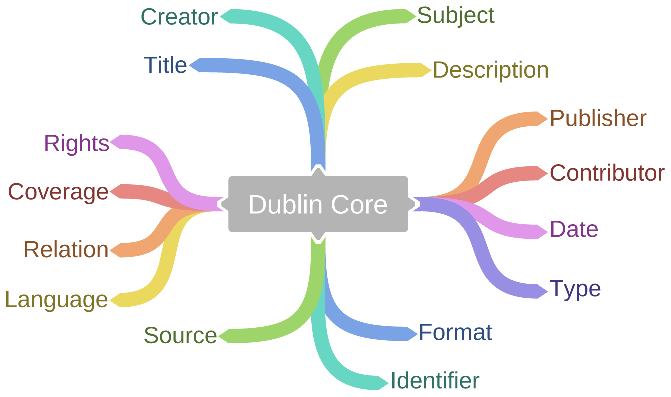
\includegraphics[width=0.5\textwidth]{bilder/doku_dublinCore}
  \end{center}
  \caption{Die 15 Kernfelder von Dublin Core Version 1.1. (Grafik erstellt mit coggle.it.)}
  \label{doku_dublinCore}
\end{wrapfigure}
Für deskriptive Metadaten ist das unter ISO 15836 zertifizierte Metadatenschema \emph{Dublin Core} (in Abbildung \ref{doku_dublinCore}) am weitesten verbreitet. Es verfügt in der Version 1.1 über folgende 15 Kernfelder: \emph{Title} (Titel) -- \emph{Creator} (Ersteller) -- \emph{Subject} (Thema) -- \emph{Description} (Beschreibung) -- \emph{Publisher} (Verleger) -- \emph{Contributor} (Mitwirkender) -- \emph{Date} (Datum) -- \emph{Type} (Typ) -- \emph{Format} (Format) -- \emph{Identifier} (Identifikator) -- \emph{Source} (Quelle) -- \emph{Language} (Sprache) -- \emph{Relation} (Beziehung) -- \emph{Coverage} (Umfang) -- \emph{Rights} (Rechte).

Im Laufe der Jahre wurde dieses grundlegende Set noch erweitert. Das aktuelle Set, "`\emph{The Dublin Core Metadata Initiative (DCMI) Metadata Terms}"', und die Beschreibung der einzelnen Attribute kann \href{http://dublincore.org/documents/dcmi-terms/}{online}\footnote{\href{http://dublincore.org/documents/dcmi-terms/}{http://dublincore.org/documents/dcmi-terms/}} abgerufen werden.

Eine besondere Relevanz im archäologischen und altertumswissenschaftlichen Kontext haben folgende Standards erlangt:
\begin{itemize}
	\item Online AccesS to the Index of archaeological investigationS (OASIS), veröffentlicht von English Heritage. Es wurde für den Nachweis von archäologischen Projekten und Maßnahmen in Großbritannien entwickelt. Das Schema liegt aktuell in Version 1.3 vor. Neben den in der Abbildung \ref{abb:doku_oasisProject} dargestellten fünf Themenbereichen können auch weitere spezielle Angaben wie etwa zu Arealen, Geophysik, Geologie und Artefakten gemacht werden.
	\begin{figure}[h!bt]
		\begin{center}
			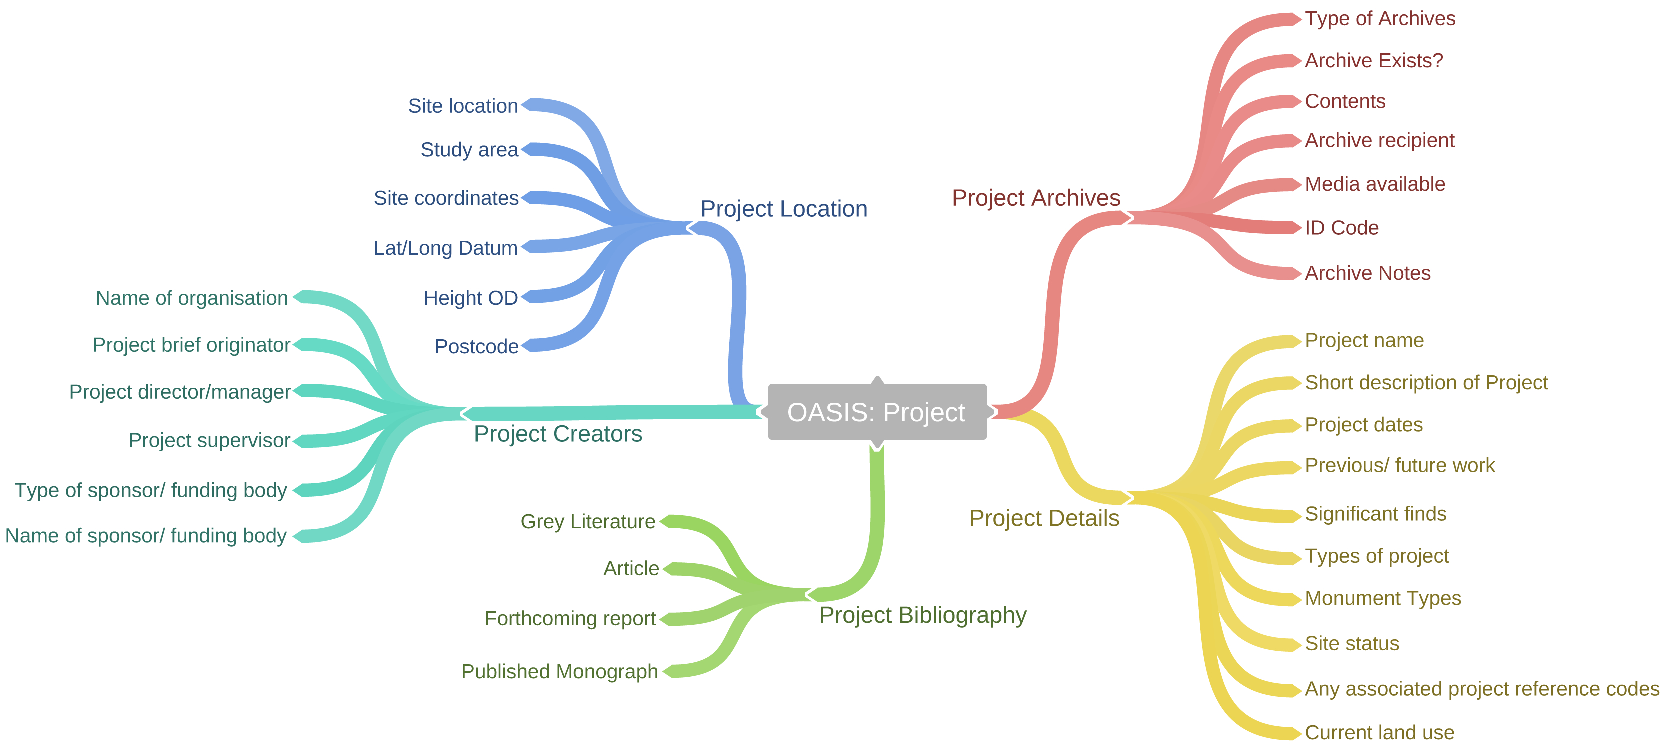
\includegraphics[width=\textwidth]{bilder/doku_oasisProject}
		\end{center}
		\caption{OASIS in Version 1.3. Neben den abgebildeten Themenbereichen sind auch Attribute für weitere spezialisiertere Informationen vorgesehen. (Grafik erstellt mit coggle.it.)}
		\label{abb:doku_oasisProject}
\end{figure}
	\item Archäologischer DateneXport-Standard (ADeX), wurde von der "`Kommission Archäologie und Informationssyteme"' beim Verband der Landesarchäologen entwickelt. Der Standard wurde für den Austausch archäologischer Fachdaten zwischen Landesämtern und anderen Institutionen erarbeitet. Die aktuelle in Abbildung \ref{abb:doku_ADeX} dargestellte Version ist 2.0, die auch den Austausch von komplexen Geometrien mittels externer Geometriedaten (SHP oder MIF) ermöglicht. ADeX ist bewusst als einfaches Austauschformat mit den Teilen "`Generelles"', "`Georeferenz"' und  "`Typ und Zeit"' unter Berücksichtigung internationaler Standards, wie etwa CIDOC-CRM, gestaltet. Dies gewährleistet eine hohe Austauschbarkeit.
	\begin{figure}[h!bt]
		\begin{center}
			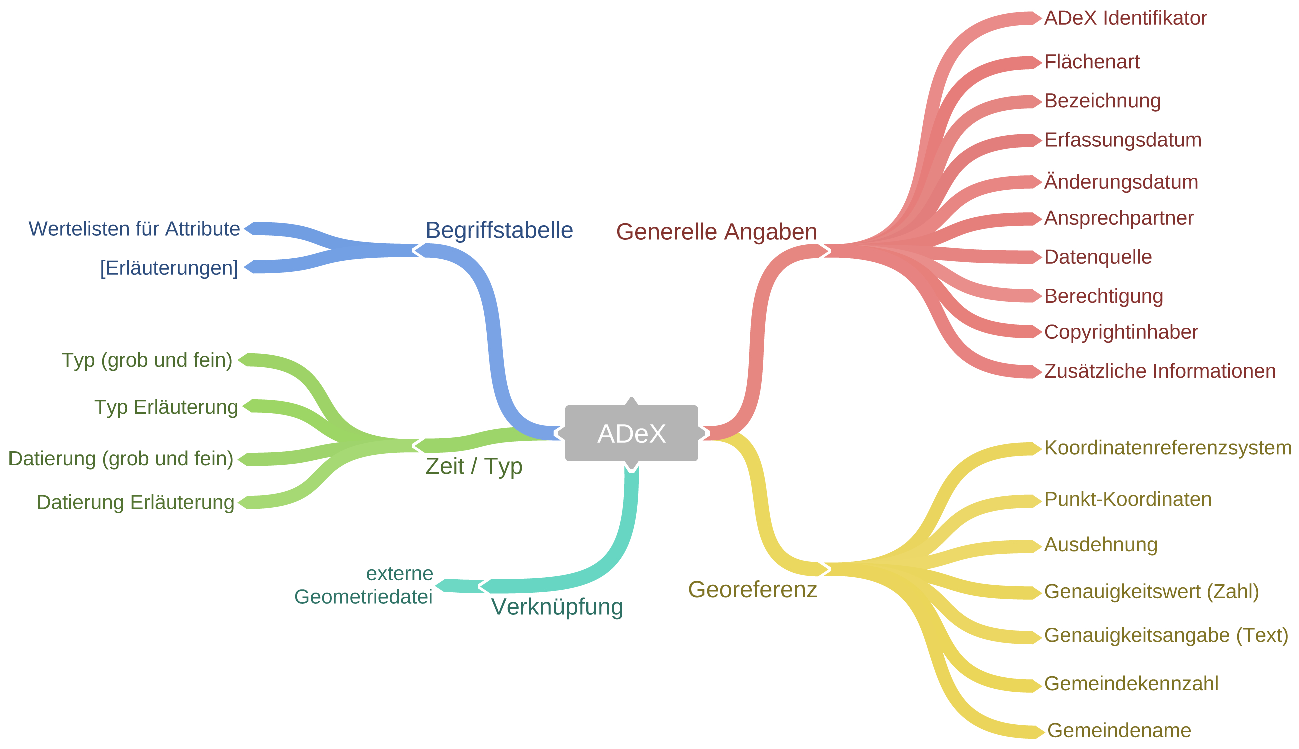
\includegraphics[width=\textwidth]{bilder/doku_ADeX}
		\end{center}
		\caption{ADeX in Version 2.0, das für eine hohe Kompatibilität auf detailliete Informationen verzichtet. (Grafik erstellt mit coggle.it.)}
		\label{abb:doku_ADeX}
\end{figure}
	\item Connecting Archaeology and Architecture in Europeana (CARARE) in Version 2.0. Es wurde als archäologiespezifisches Datenmodell unter Berücksichtigung verschiedener europäischer Standards von Europeana und dem Project 3D-ICONS entwickelt. Die Abbildung \ref{abb:doku_CARARE} verdeutlicht, dass in dem Schema Informationen zur Sammlung (\emph{Collection information}), zum physischen Objekt (\emph{Heritage asset}), zur digitalen Ressource (\emph{Digital resource}) und zur Aktivität (\emph{Activity}) definiert werden.
	\begin{figure}[h!tb]
		\begin{center}
			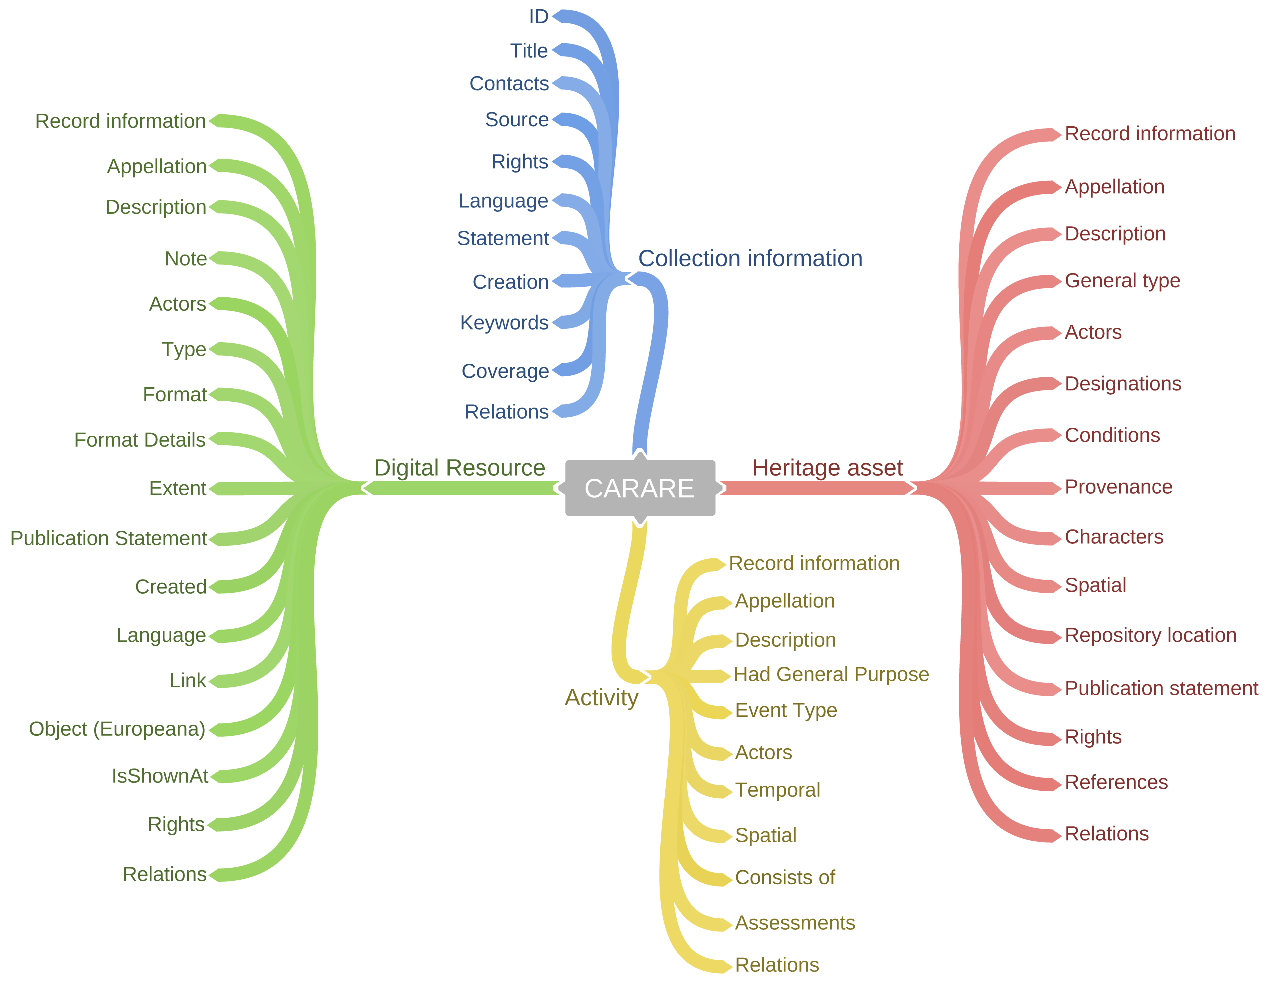
\includegraphics[width=0.9\textwidth]{bilder/doku_CARARE}
		\end{center}
		\caption{CARARE 2.0. (Grafik erstellt mit coggle.it.)}
		\label{abb:doku_CARARE}
\end{figure}
\item Das Metadatenschema von IANUS in Abbildung \ref{abb:doku_IANUS} wurde ebenfalls für Daten aus dem Bereich der Archäologien und Altertumswissenschaften entwickelt und orientiert sich an bereits vorhandenen Standards.
\begin{figure}[h!bt]
		\begin{center}
			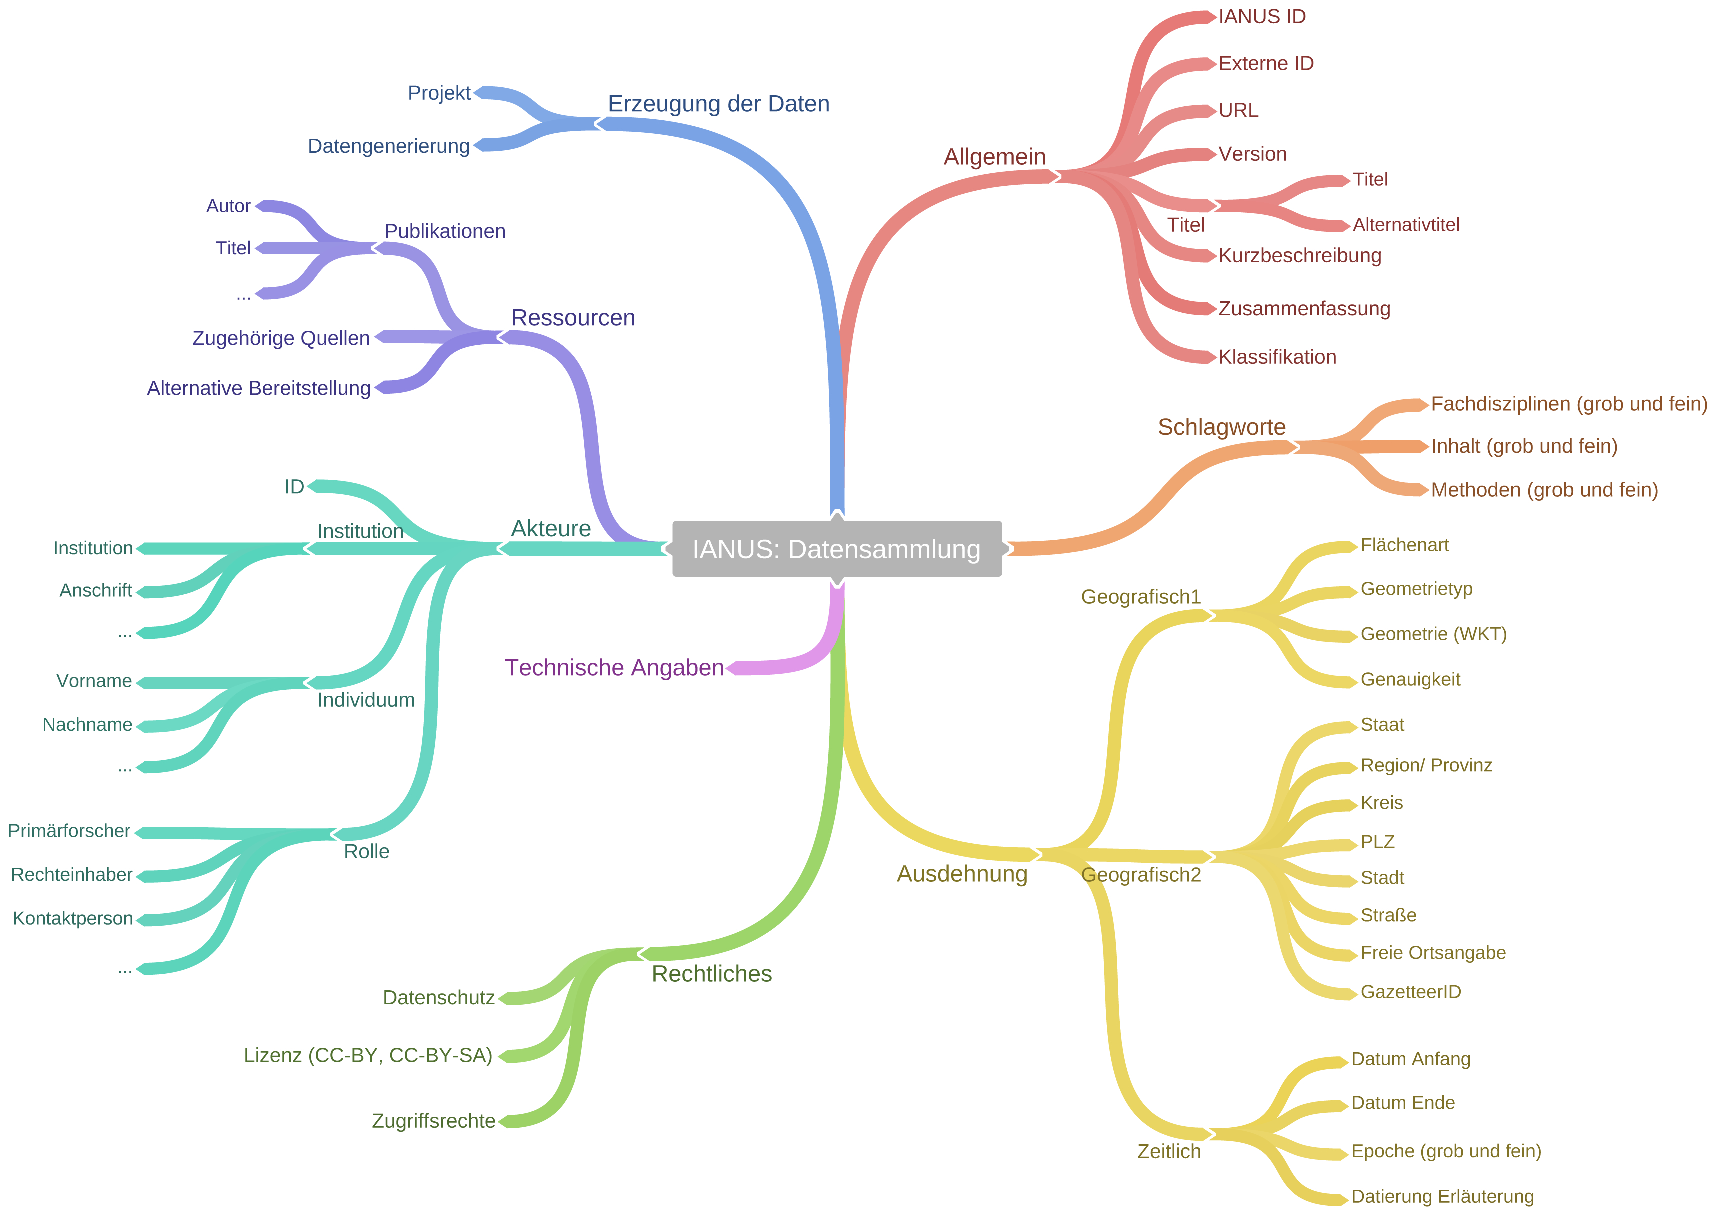
\includegraphics[width=\textwidth]{bilder/doku_IANUS}
		\end{center}
		\caption{Eine vereinfachte Darstellung des Metadatenschemas von IANUS. (Grafik erstellt mit coggle.it.)}
		\label{abb:doku_IANUS}
\end{figure}
\end{itemize}

Darüberhinaus gibt es weitere internationale Standards und institutionelle Vorgaben:
\begin{itemize}
	\item CIDOC Conceptual Reference Modell (CIDOC CRM) wurde von der Arbeitsgruppe "`Dokumentationsstandards"' im Internationalen Komitee für Dokumentation (CIDOC) des internationalen Museumsverbandes (ICOM) erarbeitet. Es dient der Strukturierung und formalen Beschreibung von Informationen, Konzepten und Relationen im Bereich des Kulturerbes. Seit 2006 ist CIDOC CRM unter ISO 21127 standardisiert. Für CIDOC-CRM gibt es zusätzlich die im Rahmen von ARIADNE entwickelten Erweiterungen CRMarchaeo, CRMba, CRNdig und CRMgeo, die eine Relevanz für die Archäologie haben. Sie werden in dem Ariadne Reference Model zusammengefasst.
	\item Das Lightweight Information Describing Objects (LIDO) wurde als Austauschformat für bewegliche Objekte in Museen von Arbeitsgruppen innerhalb von CIDOC entwickelt.
	\item Historic Environment Records oder MIDAS Heritage aus Großbritannien.
	\item Vorgaben verschiedener Denkmalämter. Weitere Informationen dazu sind in dem Abschnitt "`Grabungsdokumentation"' ab Seite \pageref{grabungsdokumentation} zu finden.
\end{itemize}


%##################################################################################

\subsection{Kontrollierte Vokabulare, Thesauri und Normdaten}
Damit Metadaten möglichst sinnvoll genutzt und maschinell verarbeitet werden können, sollten neben klar definierten Metadatenschemata auch möglichst einheitliche Begriffe und homogene Beschreibungen verwendet werden. Nur wenn gleiche Dinge auch mit den gleichen Begriffen benannt werden, ist es möglich vollständige und präzise Suchergebnisse zu erhalten oder vergleichbare Daten richtig miteinander zu verknüpfen. Die Vorgabe und Definition von festen Begriffen und Regeln hilft zudem, Mehrdeutigkeiten und Redundanzen zu vermeiden, etwa wenn eine Zeichenkette verschiedene Bedeutungen besitzen kann (z. B. Abakus als Rechenhilfsmittel oder als architektonischer Abschluss eines Kapitells), ein identischer Sachverhalt durch unterschiedliche Worte erfasst werden kann (z. B. Survey und Oberflächenbegehung) oder die Form der Angabe variieren kann (z. B. ein Datum in der Form 12.03.2012 oder 2012-03-12).
 
Das geeignete Mittel zur Vereinheitlichung der sprachlichen Vielfalt sind sogenannte kontrollierte oder normierte Vokabulare, die entweder einfache Wortlisten oder strukturierte Thesauri sein können, in denen Wörter zusammen mit ihrem semantischen Kontext verwaltet werden. Diese "`terminologische Kontrolle"' kann in unterschiedlicher Weise systematisiert und implementiert sein. 

Beispielsweise können innerhalb eines Projektes alle zu verwendenden Begriffe unter allen Beteiligten abgestimmt, klar fachlich definiert, voneinander abgegrenzt und in strukturierter Form dokumentiert werden. Diese Absprachen können dann in einem zentralen Textdokument als Projektleitfaden abgelegt oder in einer Datenbank als Felder umgesetzt werden, die nur eine begrenze Auswahl von Begriffen zur Beschreibung eines spezifischen Sachverhaltes zulassen (z. B. für das Attribut Filmart nur die Werte "`Diapositiv (Farbe)"', "`Negativfilm (Farbe)"', "`Negativfilm (SW)"' und "`Digital"').

Besser eignen sich jedoch etablierte, standardisierte, globale Vokabulare, Thesauri oder Normdateien. Sie weisen oft eine thematische, fachspezifische oder institutionelle Ausprägung auf und werden von maßgeblichen Einrichtungen kontinuierlich gepflegt. Dazu gehören beispielsweise Normdateien zur Katalogisierung aus dem Bibliotheksbereich, Personennormdateien oder Thesauri zur eindeutigen Identifizierung von geografischen Orten oder Zeitbegriffen. 

Diese globalen Systeme bieten nicht nur eine feste Bezeichnung und eine Definition eines Begriffes oder des diesem zugrunde liegenden Konzeptes, sondern auch alternative und gegebenenfalls mehrsprachige Benennungen und eine eindeutige Kennung zur Identifizierung des Begriffes. So kann beispielsweise der Ort "`Alexandria"' (\href{http://www.geonames.org/361058/alexandria.html}{361058}) in Ägypten von dem Ort "`Alexandria"' (\href{http://www.geonames.org/4744091/alexandria.html}{4744091}) in den USA mittels der in den Klammern angegebenen Kennungen aus GeoNames unterschieden werden.

Bereits existierende Thesauri und Vokabulare sollten bei der Vergabe von Metadaten berücksichtigt und angewendet werden, um den späteren elektronischen Austausch, also die Interoperabilität, der eigenen Daten mit anderen Systemen erheblich zu vereinfachen. Wenn Ressourcen in mehreren Sprachen vorliegen und entsprechend multilingual beschrieben werden sollen, müssen die genutzten Wörterbücher, Thesauri und Schlagwortsysteme äquivalente Begriffe in mehreren Sprachen abbilden.

Für die systematische Erfassung archäologischer und allgemeiner Begriffe existieren folgende Vokabulare:
\begin{itemize}
	\item Art \& Architecture Thesaurus (AAT) wurde Ende der 1970er von dem Getty Research Institute entwickelt, um die Katalogisierungsprozesse in Kunstbibliotheken und im Museumsbereich zu unterstützen und zu vereinheitlichen. Dieser Thesaurus wird von einer breiten Fachgemeinschaft kuratiert.
	\item Heritage Data -- Linked Data Vocabularies for Cultural Heritage führt die in England genutzten Vokabulare im Bereich kulturelles Erbe zusammen. 
	\item Wortnetz Kultur (WNK) wurde vom Landschaftsverband Rheinland ins Leben gerufen, um die Inhalte in deren verschiedenen Informationssystemen zu vereinheitlichen. Mittlerweile sind die Themen Kulturlandschaft, Archäologie, Kulturanthropologie, Denkmalpflege sowie Kunstgeschichte mit rund 15.000 Begriffen vertreten.
	\item Das DAI bietet mit iDAI.vocab (auch archwort) ein flaches multilinguales Vokabular mit Links auf den AAT. Außerdem gibt es mit dem iDAI.the"-sau"-rus ein System, das die Schlagworte aus den unterschiedlichen Thesauri der Bibliotheken zusammenführt und strukturiert.
	\item Die Encyclopedia of Life stellt eine weltweite Datenbank für Pflanzen und Lebewesen dar, die zusätzlich Fotos, Verbreitungskarten und Literaturhinweise enthält.
	\item In Wikidata werden alle strukturierten Daten aus den Systemen von WikiMedia erfasst und mit eindeutigen Identifikatoren zur Verfügung gestellt.
\end{itemize}

Für die eindeutige Identifizierung von geografischen Orten eignen sich, neben den amtlichen Gemeindekennzahlen und dem geodätischen Parameterdatensatz EPSG, folgende Ortsthesauri, sogenannte Gazetteers:
\begin{itemize}
	\item GeoNames ist ein Gazetteer, in dem vor allem moderne Orte, deren alternative Bezeichnungen und geografischen Koordinaten systematisch erfasst werden. Die Inhalte stammen von engagierten Nutzern weltweit.
	\item Getty Thesaurus of Geographic Names (TGN) wurde 1987 von dem Getty Research Institute ins Leben gerufen, um ebenfalls deren Katalogisierungsprozesse in Kunstbibliotheken und im Museumsbereich zu unterstützen und zu vereinheitlichen.
	\item Das DAI betreibt mit dem iDAI.gazetteer einen Gazetteer für die eindeutige Adressierung von antiken Orten, in dem außerdem auch die Eintragungen in GeoNames berücksichtigt werden.
	\item Pleiades ist ebenfalls ein Gazetteer für antike Orte mit einem Schwerpunkt auf der griechischen und römischen Antike, dessen Inhalt durch jeden Nutzer erweitert oder korrigiert werden kann.
\end{itemize}

Auch für Zeitbegriffe gibt es kontrollierte Vokabulare:
\begin{itemize}
	\item PeriodO ist ein Gazetteer für Zeitepochen. Neben der zeitlichen Information wird auch die geografische Verbreitung der jeweiligen Epoche erfasst.
	\item iDAI.chronontology ist ein vom DAI durchgeführtes Projekt, das wie PeriodO zeitliche und geografische Informationen miteinander in Beziehung setzt.
\end{itemize}

Zur Erfassung von Informationen zu Personen oder Institutionen sollten Normdateien verwendet werden, wie beispielsweise:
\begin{itemize}
	\item Das Virtual International Authority File (VIAF) kombiniert Normdateien mehrerer Nationalbibliotheken und speichert Informationen zu Personen und Institutionen, sowie deren Publikationen.
	\item Die Open Researcher and Contributor ID (ORCID) ist eine alphanumerische Zeichenkette, die der eindeutigen Identifizierung wissenschaftlicher Autoren dient. ORCID wird von einem gemeinnützigen Gremium betrieben und Autoren müssen sich selbst registrieren, um eine ID zu bekommen.
	\item Die Gemeinsame Normdatei (GND) der Deutschen Nationalbibliothek dient primär der Katalogisierung in Bibliotheken. Neben Informationen zu Personen und Körperschaften werden auch weitere Informationen zu Konferenzen, Geografika, Sachschlagwörtern und Werktiteln verwaltet.
\end{itemize}

Wenn in Metadaten auf Publikationen verwiesen werden soll, eignen sich folgende Systeme:
\begin{itemize}
	\item Die Internationale Standardbuchnummer (engl. \emph{International Standard Book Number}, ISBN) wird zur eindeutigen Identifizierung von Publikationen verwendet. Sie ist vor allem im Buchhandel verbreitet. Für Reihen und Zeitschriften wird eine ähnliche Nummer, die ISSN (Internationale Standardnummer für fortlaufende Sammelwerke, engl. \emph{International Standard Serial Number}) verwendet.
	\item Für in Deutschland veröffentlichte Medienwerke gibt es eine Ablieferungspflicht bei der Deutschen Nationalbibliothek, weshalb die dort vergebenen  eindeutigen Kennungen ebenfalls zur Identifizierung verwendet werden können.
	\item Für archäologische und altertumswissenschaftliche Publikationen eignen sich auch die Identifikatoren aus iDAI.bibliography (Zenon), in dem die umfangreichen Bestände aller DAI Bibliotheken nachgewiesen werden.
\end{itemize}

%##################################################################################
\label{metadatenSpeicherung}
\subsection{Speicherung von Metadaten}
Für eine strukturierte Speicherung von Metadaten gibt es verschiedene Möglichkeiten und Wege, die einerseits von dem Zeitpunkt (synchron mit der Datenerhebung oder im Nachhinein) und andererseits von der Art der Metadatenerfassung (manuell oder automatisiert) abhängen. 

Grundsätzlich sollten Metadaten so früh wie möglich, also bereits bei der Generierung von neuen digitalen Objekten oder am Anfang eines neuen Forschungsvorhabens vergeben werden, auch wenn diese noch nicht vollständig angegeben werden können. Somit wird vermieden, dass Informationen im Nachhinein nicht mehr nachgetragen werden können, da sie vergessen wurden oder sich nicht mehr ermitteln lassen. Eine regelmäßige Aktualisierung und kontinuierliche Metadatenpflege ist ratsam und für manche Daten, wie etwa 3D-Scans oder Geodaten auch erforderlich.

Abhängig vom verwendeten Dateiformat können Metadaten auch direkt in eine Datei integriert werden. Dies kann teilweise automatisiert erfolgen, wie beispielsweise bei digitalen Fotos. Hier werden von der Kamera automatisch technische Angaben zu Dateiformat, Verschlusszeit, Blendenöffnung, Farbinformationen usw. direkt in der Bilddatei hinterlegt. Je nach Gerät können über die Voreinstellungen auch deskriptive Informationen wie Fotograf, Aufnahmedatum, Land etc. hinzugefügt werden. Ähnliche Verfahren zur automatischen Metadatenerzeugung sind auch bei Vermessungsgeräten üblich. Die durch Geräte generierten Metadaten werden unmittelbar in einem besonderen Bereich und auf standardisierte Weise in der resultierenden Datei gespeichert, etwa bei Fotos im Format Exif im Header der Datei.

Mit Hilfe von editierbaren Dateieigenschaften können auch in anderen Dateiformaten, wie etwa DOCX, ODT oder PDF, Metadaten direkt im Header gespeichert werden. Dabei ist jedoch eine manuelle Eingabe mit Hilfe der passenden Software erforderlich. Diese Informationen können über die Eigenschaften einer Datei angezeigt und teilweise verändert und ergänzt werden, was in Abbildung \ref{eigenschaftenAcrobat} für ein PDF-Dokument zu sehen ist. Bei der Auswahl von Anwendungen sollte darauf geachtet werden, ob diese spezifischen Metadaten entweder als separate Datei exportiert oder ob sie mit den Dateien, in denen sie enthalten sind, auch unabhängig von der ursprünglichen Software geöffnet werden können.

\begin{figure}[t!]
  \begin{center}
    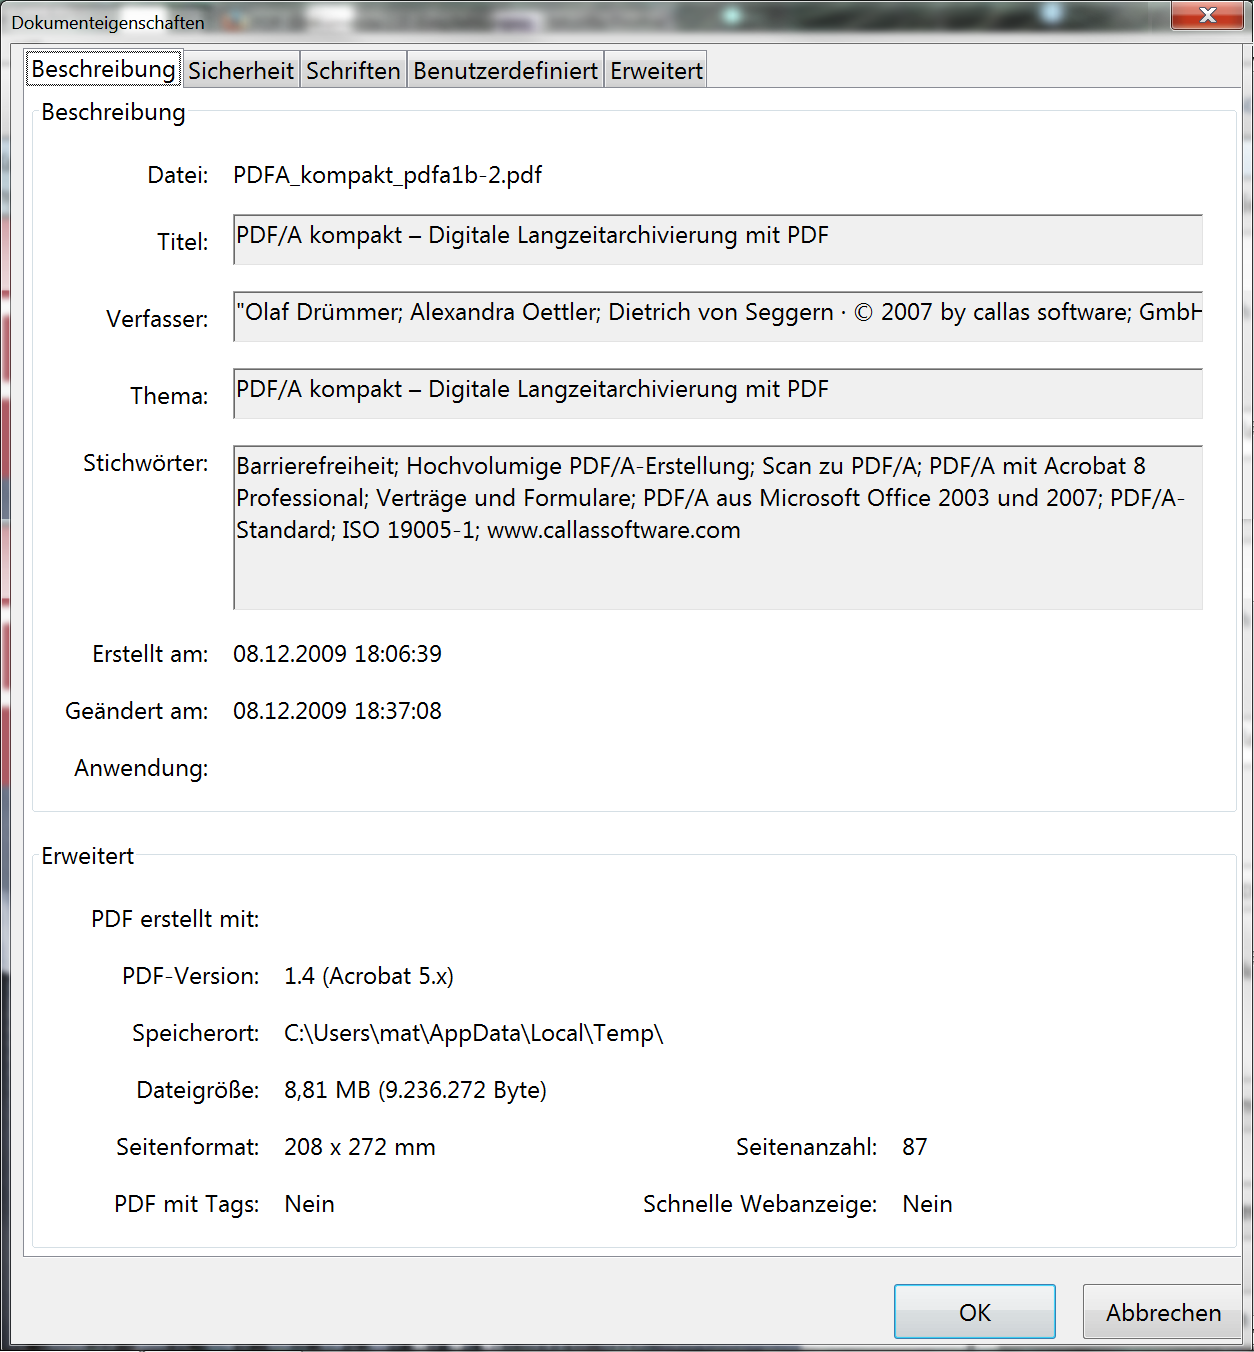
\includegraphics[width=0.9\textwidth]{bilder/doku_AdobeEigenschaften}
  \end{center}
  \caption{Beispiel der Metadaten eines PDF-Dokumentes im Programm Adobe Reader. Die Metadaten können unter "`Datei > Eigenschaften"' angezeigt und verändert werden.}
  \label{eigenschaftenAcrobat}
\end{figure}

Bei textbasierten (insbesondere XML-basierten) Dateiformaten oder Textdateien, die Auszeichnungssprachen verwenden (wie etwa SVG-, HTML- oder XML-Dateien), können Metadaten leicht mittels Auszeichnungselementen im Header der Datei integriert werden. Konkrete Hinweise für die Bearbeitung und Ergänzung von Metadaten für bestimmte Dateiformate sind in den entsprechenden Abschnitten im Kapitel Dateiformate ab Seite \pageref{dateiformate} zu finden. Auch Hinweise für die Extraktion von Metadaten in separate Dateien sind ebenfalls in den entsprechenden Abschnitten zu finden.

Für Dateiformate, in denen kein eigener Metadatenbereich vorgesehen ist, oder für übergeordnete projekt- und methodenbezogene Metadaten, ist eine Speicherung in separaten Dateien oder Systemen erforderlich. Hierfür eignen sich Tabellen und Datenbanken, da diese die Erfassung mithilfe spezifischer Eingabemasken, einer gezielten Suche und einer strukturierten Sicherung von Metadaten erleichtern. Zusätzlich erlauben sie eine (Teil-)Automatisierung der Metadaten, wie etwa die automatische Speicherung des Datums der letzten Bearbeitung eines Datensatzes und den Namen des Bearbeiters. Ein weiterer Vorteil der Erfassung von Metadaten in Tabellen oder Datenbanken besteht in der effizienten Bearbeitung von Merkmalen, die für mehrere Dokumente identisch sind, wie beispielsweise der gleiche Maßstab für alle Zeichnungen eines Projektes.

Bei der Speicherung von Metadaten in separaten Dateien muss in besonderer Weise darauf geachtet werden, dass die Beziehungen zwischen beiden Einheiten eindeutig und aktuell sind. Wird etwa bei den Metadaten der Name einer Datei zur Identifizierung verwendet, muss sichergestellt werden, dass dieser einmalig ist (ggf. in Kombination mit seinem Speicherort) und dass im Falle der Umbenennung der Datei der Eintrag auch bei den Metadaten aktualisiert wird.

Die Erfassung von Metadaten in einer Freitextdatei sollte vermieden werden, da diese meist nicht automatisiert durch Computer überprüft und verarbeitet werden können.

Bei Dokumenten mit Textinhalt können beschreibende Metadaten auch automatisch erzeugt werden, indem nach charakteristischen Zeichenketten gesucht wird und Schlag- und Stichworte extrahiert werden. Allerdings reicht die Qualität einer automatischen Erschließung bislang nicht an eine manuelle und intellektuelle Metadatenvergabe heran, da maschinell nicht nur sinnvolle Deskriptoren herausgefiltert werden.

Für die Übergabe von Dateien und Metadaten an ein Langzeitarchiv gilt die Empfehlung, die Metadaten sowohl in den Originaldateien selbst als auch in einem separaten, strukturierten und textbasierten Dokument vorzuhalten: in den Originaldateien selbst, um keine verwaisten, also undokumentierten Werke zu erzeugen, und als separate Textdatei, um eine automatisierte Verarbeitung und den Austausch von Referenzangaben zu vereinfachen.
\subsection{Metadaten in der Anwendung}
\label{Metadaten-anwendung}
\paragraph{Projektbezogene Metadaten}
Die wichtigsten Metadaten, die für die Beschreibung eines Projektes oder einer Dokumentensammlung erforderlich sind, werden in der folgenden Tabelle abgebildet und knapp definiert. Sie geben einen Überblick über einen größeren, zusammenhängenden Datenbestand und beschreiben den fachlichen Kontext in dem dieser entstanden ist. Vergleichbar einem Bibliothekskatalog liegt die Hauptfunktion dieser Metadaten darin, dass externe Personen ein Projekt oder eine dessen digitale Daten über Web-Portale und Suchmaschinen finden und einordnen können. Darüber hinaus enthalten sie rechtliche Informationen, die für den weiteren Umgang mit den Daten wichtig sind. 

Die hier vorgestellten Eigenschaften basieren auf dem Dublin Core Metadata Schema und den Angaben, wie sie vom ADS in den UK und tDAR in den USA erhoben werden, um einen zukünftigen Austausch zu vereinfachen. Ein darauf aufbauendes ausführliches Metadatenschema, das auch die Grundlage für die Archivierung von Projektdaten bei IANUS bildet, sowie ausgefüllte Beispielformulare sind in dem Kapitel Archivierung von Forschungsdaten in IANUS ab Seite \pageref{archivierungIANUS} zu finden.

\begin{center}
	\begin{longtable}{L{0.25\textwidth} p{0.68\textwidth}}
		\toprule
		Bezeichnung & Kurzdefinition\\ \midrule \endfirsthead
		\multicolumn{2}{l}{\footnotesize Fortsetzung der vorhergehenden Seite}\\
		\toprule
		Bezeichnung & Kurzdefinition\\ \midrule \endhead
		\bottomrule \multicolumn{2}{r}{{\footnotesize Fortsetzung auf der nächsten Seite}} \\
		\endfoot
		\bottomrule 
		\endlastfoot

		Identifizierung -- Projekttitel & Verbindliche Kurzbezeichnung des Projektes.\\
		Identifizierung -- Alternativtitel & Ggf. alternative Titel für ein Projekt.\\
		Identifizierung -- Projektnummer(n) & Nummern oder Kennungen, die z.B. innerhalb der durchführenden Organisation oder von Mittelgebern verwendet werden, um das Projekt eindeutig identifizieren zu können.\\
		Kurzbeschreibung & Knappe Angaben zur Fragestellung, zum Verlauf und Ergebnis des Projektes sowie Skizzierung der Datensammlung (insgesamt ca. 100-300 Worte)\\
		Schlagworte -- Fachdisziplinen & Stichworte, die die beteiligten Disziplinen und Fächer benennen. Sofern die Stichworte auf publizierten Standards oder internen Thesauri beruhen, müssen diese mitangegeben werden.\\
		Schlagworte -- Inhalt & Stichworte, die den Inhalt der Datensammlung benennen., z. B. zu Materialgruppen, Fundstellen-Klassifizierung, Quellenarten,  Kulturgruppen etc. Sofern die Stichworte auf publizierten Standards oder internen Thesauri beruhen, müssen diese mitangegeben werden.\\
		Schlagworte -- Methoden & Stichworte, die die eingesetzten Forschungsmethoden beschreiben. Sofern die Stichworte auf publizierten Standards oder internen Thesauri beruhen, müssen diese mitangegeben werden.\\
		Ausdehnung -- Geografisch-1 & Detaillierte Angaben zur räumlichen Ausdehnung oder zum Fundort des untersuchten Gegenstandes mittels geografischer Koordinaten. Die maximale Ausdehnung kann als Bounding Box angegeben werden.\\
		Ausdehnung -- Geografisch-2 & Sprachliche Beschreibung des untersuchten Gegenstandes mittels Ortsangaben mit Land, Stadt, Kreis, Straße, Gemarkung etc. Sofern Namen sich im Lauf der Zeit geändert haben, dies gesondert vermerken. Sofern eine Referenz zu einer Geo-Ressource oder einem Gazetteer existiert, sollte diese ebenfalls angegeben werden.\\
		Ausdehnung -- zeitlich & Chronologische Angaben zum untersuchten Gegenstand, entweder als Periodenbezeichnung und/oder mit groben/genauen Jahresangaben. Sofern die Stichworte auf publizierten Standards oder internen Thesauri beruhen, müssen diese mitangegeben werden.\\
		Primärforscher -- Person & Personen, die entweder für das Projekt als Ganzes, für das Datenmanagement oder für die Erzeugung bestimmter Datenarten zentral bzw. verantwortlich sind. Hier ist eine Kontaktadresse erforderlich und die aktuelle/letzte institutionelle Zugehörigkeit, damit die Personen bei Rückfragen erreicht werden kann.\\
		Eigentümer -- Organisation & Organisation, der die unter "`Primärforscher"' genannten Personen angehören, oder die nach Ausscheiden derselben für die Daten verantwortlich ist, im weitesten Sinne also Eigentümer der Daten ist. Hier ist eine Kontaktadresse erforderlich, damit die Organisation bei Rückfragen erreicht werden kann.\\
		Finanzierung & Nennung der Organisation(en) / (Dritt-)Mittelgeber, durch die das Projekt finanziert wurde. Es sollte jeweils der Zeitraum der Finanzierung angegeben werden.\\
		Veröffentlichung -- Projektdaten & Wenn die hier beschriebene Datensammlung des Projektes bereits an anderer Stelle veröffentlicht / online gestellt wurde, bitte entsprechende Angaben machen, z. B. durch Nennung der Organisationen, Datenarchive, Online-Ressourcen etc.\\
		Veröffentlichung -- Ergebnisse & Analoge oder digitale Publikationen zu Ergebnissen des Projektes oder zur Datensammlung des Projektes, ausführliche bibliographische Angaben (ohne fachspezifische Abkürzungen) unter Nennung des Verlages erforderlich.\\
		Dauer -- Projekt & Anfangs- und Enddatum des Projektes.\\
		Dauer -- Datenbestand & Anfangs- und Enddatum der Erzeugung oder Verarbeitung digitaler Daten im Rahmen des Projektes.\\
		Rechtliches -- Urheberrechte & Name des Inhabers der Urheber-, Nutzungs- und Verwertungsrechte; i. d. R. die Organisation, an der der Primärforscher beschäftigt war.\\
		Rechtliches -- Lizenzgeber & Angabe der Person, die i. d. R. als Vertretung für eine Organisation für die Lizenzierung von Daten zur Nachnutzung verantwortlich und berechtigt ist, einen Datenübergabevertrag abzuschließen.\\
		Rechtliches -- Datenschutz & Angaben, ob in der Datensammlung datenschutzrelevante Informationen enthalten sind. Wenn ja, in welchem Umfang.\\
		Quellen -- Ältere & Ältere Quellen oder existierende Ressourcen, auf denen die Daten aufbauen.\\
		Quellen -- Zugehörige & Sofern während des Projektes Informationen, Datensammlungen, (un-)publizierte Dokumente, Online-Ressourcen etc. verwendet oder erzeugt wurden, die nicht Teil der hier beschriebenen Datensammlung sind, aber für deren Verständnis wichtig sind, bitte entsprechende Angaben zu Art und Umfang dieser Quellen machen.\\
		Sprache & Die in den Dokumenten und Dateien verwendete(n) Sprache(n). Sprachkennungen nach ISO 639 angeben.\\
		Art der Daten & Kurzcharakterisierung der Daten, z. B. ob es sich um Rohdaten, verarbeitete Daten, Interpretationen, Ergebnisse, Abschlussberichte etc. handelt.\\
		Vollständigkeit & Aussagen zur Vollständigkeit der Projektdaten, z. B. ob bestimmte Datenarten noch fehlen und warum.\\
		Dateiformate & Auflistung der Dateiformate, die in der Datensammlung vorkommen, ggf. unter Nennung der verwendeten Programme und Zeichenkodierungen.\\
		Zugriffsrechte & Festlegung der gewünschten Zugriffsrechte für die Daten, sofern diese für den gesamten Projekt-Datenbestand gelten sollen; differenzierte Regelungen müssen auf Dateiebene vorgenommen werden.\\
		Signatur Metadaten & Angabe darüber, wer die o. g. Metadaten wann ausgefüllt hat.\\
		\bottomrule
	\end{longtable}
\end{center}

\paragraph{Dateibezogene Metadaten}
Bei dieser Art von Metadaten handelt es sich um technische und inhaltliche Informationen, die Nutzern verständlich machen, wie einzelne Dateien innerhalb eines Projektes oder einer Datensammlung beschaffen sind und welche Möglichkeiten der Nachnutzbarkeit sie beinhalten. 

Dateibezogene Metadaten sind abhängig von dem Format, dem Inhalt und der Methode, mit denen die Dateien erzeugt wurden. Beispielsweise sind für Rastergrafiken, die durch digitale Fotografie entstanden sind, andere Angaben erforderlich (Fotograf, Aufnahmedatum, Aufnahmeort, abgelichtetes Objekt etc.) als für Rasterdateien, die durch geophysikalische Messungen erzeugt wurden (Koordinaten, Messgerät, Genauigkeit, Datum etc.). Zusätzliche spezifische Angaben, die für bestimmte Dateiformate empfohlen werden, sind in den verschiedenen Kapiteln zu den jeweiligen Formaten ab Seite \pageref{dateiformate} beschrieben.

Es gibt jedoch dateibezogene Metadaten, die unabhängig von Format, Inhalt und Methode für alle Einzeldateien gleichermaßen relevant und notwendig sind. Zu diesen Metadaten gehören neben den Angaben zu Dateiname, Dateiformat, Dateiversion, Titel, Beschreibung und Ersteller auch Informationen zur verwendeten Soft- und Hardware, Versionierung, zu rechtlichen Aspekten und Verweise auf weitere relevante Dateien.

Auch wenn es in der Theorie wünschenswert ist, diese Angaben sowie die zugehörigen spezifischen Angaben zu Methoden und Dateiformaten für jede Datei einzeln zu erfassen, so zeigt die Praxis, dass es häufig ausreichend ist, einen Metadatensatz für Gruppen von Dateien anzulegen, wenn diese das gleiche Format oder die gleichen inhaltlichen Eigenschaften aufweisen. 

\begin{center}
	\begin{longtable}{L{0.25\textwidth} p{0.68\textwidth}}
		\toprule
		Bezeichnung & Kurzdefinition\\ \midrule \endfirsthead
		\multicolumn{2}{l}{\footnotesize Fortsetzung der vorhergehenden Seite}\\
		\toprule
		Bezeichnung & Kurzdefinition\\ \midrule \endhead
		\bottomrule \multicolumn{2}{r}{{\footnotesize Fortsetzung auf der nächsten Seite}} \\
		\endfoot
		\bottomrule 
		\endlastfoot
		
		Identifikator, Dateiname & Eindeutiger Name der Datei.\\
		Dateiformat & Format, in dem die Datei abgespeichert ist.\\
		Urheber & Name des Verfassers oder Erstellers der Datei.\\
		Titel & Titel der Datei, nicht der Dateiname.\\
		Beschreibung & Beschreibung des Inhalts der Datei. \\
		Schlagworte & Schlagworte, wie etwa Periode, Fundstelle oder charakteristische Merkmale. Wenn vorhanden, angemessene Thesauri verwenden.\\
		Software -- Dateierstellung & Software, mit der die Datei erstellt wurde.\\
		Hardware -- Dateierstellung & Hardware, mit der die Datei erstellt wurde, v. a. bei technischen Geräten wie Kameras, GPS-Geräten, Vermessungsinstrumenten, Laserscanner etc.\\
		Betriebssystem -- Dateierstellung & Betriebssystem, das verwendet wurde als die Datei erstellt wurde.\\
		Erstellungsdatum & Datum, an dem die Datei erstellt wurde. Datum und Zeit in UTC nach ISO 8601.\\
		Letzte Aktualisierung & Datum, an dem die Datei zuletzt bearbeitet wurde. Datum und Zeit in UTC nach ISO 8601.\\
		Dateiversion & Angabe der Versionsnummer der Datei.\\
		Weitere Dateien & Referenzen auf Dateien, die für das Verständnis einer anderen Datei zentral sind, insbesondere für zusammenhängende, komplexe Dateien oder wenn auf eine Ursprungsdatei verwiesen werden soll.\\
		Sprache & Sofern schriftliche Inhalte vorhanden sind, die Sprache angeben. Sprachkennungen nach ISO 639 angeben.\\
		Copyright-Angaben & Angaben zur Person oder Einrichtung, die das Copyright oder die Lizenzrechte an der Datei oder deren Inhalt besitzt.\\
		\bottomrule
	\end{longtable}
\end{center}

\paragraph{Methodenbezogene Metadaten}
Jede Fachdisziplin innerhalb der Altertumswissenschaften verfügt über spezifische Forschungsmethoden. Auch diese haben Einfluss auf Umfang, Art, Struktur und Inhalt digitaler Objekte, da sie bei verschiedenen Arbeitsweisen und technischen Geräten unterschiedlich ausfallen. Daher sollten methodenbezogene Metadaten ebenfalls dokumentiert werden, insbesondere wenn mehrere Zwischenstände einer Prozesskette archiviert und Dritten zur Verfügung gestellt werden sollen. Je nach Genauigkeit der Methodenbeschreibung kann sie sich sowohl auf eine Einzeldatei als auch auf mehrere Dateien gleichen Typs beziehen.

Die Angabe der methodenbezogenen Metadaten ist wichtig, um zu beschreiben, wie die Rohdaten in prozessierte Daten überführt wurden. Außerdem kann so verstanden werden, welchen Einfluss die angewandte Methode auf das Ergebnis hat, das Ergebnis folglich zu interpretieren ist und wo Fehler zu erwarten sind.

Zusätzliche spezifische Angaben, die für bestimmte Forschungsmethoden oder Prozesse empfohlen werden, sind in den einzelnen Kapiteln des Abschnittes Forschungsmethoden ab Seite \pageref{methoden} beschrieben.

\begin{center}
	\begin{tabular}{L{0.25\textwidth} p{0.68\textwidth}}
		\toprule
		Bezeichnung & Kurzdefinition\\ \midrule
		Prozessnummer & Eindeutige Nummer eines Prozesses oder einer Methode.\\
		Prozessbeschreibung & Beschreibung des Prozesses oder der Methode. Insbesondere Beschreibung der Ausgangssituation und der Zielvorstellung.\\
		Ausgangsformat(e) & Format der Dateien, die am Anfang eines gesamten Prozesses stehen und den Ausgangspunkt bilden.\\
		Zwischenformat(e) & Format der Dateien, die im Verlauf eines Prozesses erzeugt werden und den Ausgangspunkt für weitere Prozesse bilden.\\
		Zielformat(e) & Format der Dateien, die am Ende eines Prozesses erzeugt werden.\\
		Durchführender & Person(en), die den Prozess durchgeführt hat (haben).\\
		Prozessbeginn & Datum, an dem der Prozess begonnen wurde. Datum und Zeit in UTC nach ISO 8601.\\
		Prozessende & Datum, an dem der Prozess beendet wurde. Datum und Zeit in UTC nach ISO 8601.\\
		Software & Software, mit der der Prozess durchgeführt wurde.\\
		Hardware & Hardware, auf der der Prozess durchgeführt wurde.\\
 		\bottomrule
		\bottomrule
	\end{tabular}
\end{center}


%##################################################################################
\label{grabungsdokumentation}
\subsection{Grabungsdokumentation}
Speziell für die Dokumentation von Grabungen und anderen archäologischen Maßnahmen sind weitere Metadaten erforderlich, die in der folgenden Tabelle aufgelistet sind. Dabei sollten auch die verschiedenen angewandten Methoden berücksichtigt werden, da diese ebenfalls den Umfang und die Art der Dokumentation beeinflussen. Wichtig bei einer Grabungsdokumentation ist, dass nicht nur die digitalen Daten, sondern auch die analogen Daten mit einer Dokumentation versehen sind, um beispielsweise auch Abhängigkeiten zwischen den verschiedenen Daten festzuhalten. Zum Beispiel sollten Zeichnungen mit den Befundbeschreibungen, Fotos mit den Fundstellenplänen oder Objektbeschreibungen mit den jeweiligen Objekten verknüpft sein.

\begin{center}
	\begin{longtable}{L{0.25\textwidth} p{0.68\textwidth}}
		\toprule
		Bezeichnung & Kurzdefinition\\ \midrule \endfirsthead
		\multicolumn{2}{l}{\footnotesize Fortsetzung der vorhergehenden Seite}\\
		\toprule
		Bezeichnung & Kurzdefinition\\ \midrule \endhead
		\bottomrule \multicolumn{2}{r}{{\footnotesize Fortsetzung auf der nächsten Seite}} \\
		\endfoot
		\bottomrule 
		\endlastfoot

		Fundstellenart & Angabe über die Art der Fundstelle. Mehrfachangaben sind möglich, wenn beispielsweise ein sich mit einer Siedlung überlagerndes Gräberfeld beschrieben werden soll.\\
		Maßnahmenart & Angabe über die Art der Untersuchung. Werte können beispielsweise sein: Ausgrabung, Survey, Baustellenbegleitung etc.\\
		Anlass & Angabe des Anlasses, der zur Durchführung der Maßnahme führt. Werte können beispielsweise sein: Rettungsgrabung, Notgrabung, Forschungsgrabung, Lehrgrabung etc.\\
		Grabungsmethodik & Angabe der angewandten Grabungsmethodik. Werte können beispielsweise sein: Flächengrabung, Schichtengrabung, Wheeler-Kenyon-Methode etc.\\
		Verfahren & Angabe über die angewandten Arbeitsverfahren, die nicht zu Dokumentationsverfahren gehören. Werte können beispielsweise sein: Schlämmen, Bohrung, Sieben etc.\\
		Datierung & Datierung der Fundstelle, beispielsweise anhand des archäologischen Fundmaterials. Eingruppierung in eine Epoche als relative Zeitstellung und optional als absolute Zeitangabe. Bei mehrphasigen Fundstellen werden mehrere Zeiträume angegeben.\\
		Fundstellenstatus & Angaben zum Schutzstatus einer Fundstelle.\\
		Bodenbeschaffenheit & Angabe über die natürlichen Gegebenheiten und die Bodenbeschaffenheit, die Einfluss auf die Erhaltungsbedingungen von Objekten und Strukturen haben. Werte können beispielsweise sein: Feuchtboden, Mineralboden, Unter Wasser etc.\\
		Strukturen & Verschlagwortung von aufgefundenen archäologischen Strukturen, die sich aus den Befunden ergeben.\\
		Funde & Verschlagwortung von signifikanten Fundgattungen.\\
		Richtlinie & Angaben zur Grabungs- oder Dokumentationsrichtlinie, die für die Maßnahme vorgegeben war oder gewählt wurde.\\
		Dokumentationssystem & Angabe des verwendeten Dokumentationssystems. Werte können beispielsweise sein: Stellenkartensystem, Single Context Recording, spezielle institutionelle Systeme etc.\\
		Dokumentationsmethoden & Angabe der verwendeten Dokumentationsmethoden. Werte können beispielsweise sein: Text, Foto, Zeichnung, 3D-Scan, Vermessung etc. \\
		\bottomrule
	\end{longtable}
\end{center}

Die große Zahl an Dokumentationsverfahren und Forschungsmethoden führt dazu, dass eine umfassende Grabungsdokumentation aus einer großen Menge unterschiedlicher Dokumente besteht, die folgendes enthalten sollte:
\begin{itemize}
	\item Allgemeine Angaben
	\item Grabungsplan
	\item Grabungstagebuch und Grabungsprotokoll
	\item Befundblätter und Befundliste
	\item Fundzettel und/oder Fundmeldung
	\item Fund- und Probenliste
	\item Datenbanken
	\item Dokumentation der angewandten Methoden, wie:
	\begin{itemize}
		\item Vermessungsmethoden
		\item Fotografie
		\item Photogrammetrie
		\item 3D-Scans
		\item Luftbildaufnahmen
		\item Naturwissenschaftliche Beprobung
		\item Zeichnung
		\item Allgemeine Beschreibungen
	\end{itemize}
	\item Abschlussbericht
\end{itemize}

Wie eine Grabungsdokumentation aussehen und welchen Umfang sie haben soll, wird in zahlreichen Richtlinien und Vorgaben spezifiziert, die bei der Planung des Vorhabens bereits berücksichtigt werden sollten. Dabei handelt es sich meist um Vorgaben von Landesdenkmalämtern. Online verfügbare Vorgaben sind bei den weiterführenden Informationen unter Vorgaben zur Grabungsdokumentation ab Seite \pageref{Metadaten-ListeLDA} aufgelistet.

Um die Grabungsdokumentation zu erleichtern und auch sicher zu stellen, dass alle erforderlichen Metadaten angegeben werden, sollten Vorlagen für Formulare und Checklisten bereits vor der Durchführung der Maßnahme erstellt werden. In der online verfügbaren Fassung der IT-Empfehlungen sind zu diesem Kapitel passende Vorlagen zur freien Verwendung zu finden. Darunter befinden sich eine Befundliste, eine Fotoliste, eine Fundliste, eine Geräteliste, ein Probenverzeichnis, ein Restaurierungsverzeichnis, ein Zeichnungsverzeichnis und ein Dokument zur Urheberrechtsverwaltung. Ein weiterer Anhaltspunkt sind die bereits genannten Richtlinien, sowie das Werk "`Tabellen und Tafeln zur Grabungstechnik"' von Andreas Kinne und das Grabungstechnikerhandbuch des Verbandes der Landesarchäologen. 
\newpage
\subsection{Weiterführende Informationen}
\begin{flushleft}
\quelltyp{Metadaten allgemein}
Archaeology Data Service: Guides to Good Practice -- Project Metadata \urllist{http://guides.archaeologydataservice.ac.uk/g2gp/CreateData\_1-2}

Archaeology Data Service: Project metadata for the Archaeology Data Service \urllist{https://archaeologydataservice.ac.uk/resources/images/attach/ADS_collection_level_metadata_example.pdf}

DARIAH-DE (Hrsg.) Daten- und Metadatenformate in den Fachdisziplinen. Archäologie (2015) \urllist{http://dev2.dariah.eu/wiki/pages/viewpage.action?pageId=20058856}

Deutsche Initiative für Netzwerkinformation e. V. (Hrsg.) Kompetenzzentrum Interoperable Metadaten (KIM) \urllist{http://www.dini.de/ag/standards/}

Gesis: Dokumentation und Metadaten \urllist{https://web.archive.org/web/20150928031540/http://www.gesis.org/archive-and-data-management-training-and-information-center/forschungsdatenmanagement/dokumentation-und-metadaten/}

U. Jensen -- A. Katsanidou -- W. Zenk-Möltgen, Metadaten und Standards, in: S. Büttner -- H.-C. Hobohm -- L. Müller (Hrsg.) Handbuch Forschungsdatenmanagement (Bad Honnef 2011) 83-100 \urllist{http://www.forschungsdatenmanagement.de/?page_id=2}

A. Kinne, Tabellen und Tafeln zur Grabungstechnik (Dresden 2013)\abstand

J. M. Lill, Kontrolliertes Vokabular. Wieso? Weshalb? Warum?, Fachgruppe Dokumentation im DMB: Terminologie -- das Schweizer Messer der Dokumentation (9. Mai 2012, Kunstmuseum Stuttgart) \urllist{http://swop.bsz-bw.de/volltexte/2012/1002/pdf/Lill_Textfassung_VortragDMB2012.pdf}

J. Lindenthal, Normen und Standards für Thesauri (2015) \urllist{https://www.ianus-fdz.de/it-empfehlungen/sites/default/files/NormenEmpfehlungenEntwicklungThesauri_Lindenthal.pdf}

nestor (Hrsg.) Standardisierung -- Metadaten \urllist{https://wiki.dnb.de/display/NESTOR/Metadaten}

C. Papatheodorou -- D. Gavrilis -- K. Fernie -- H. Wright -- J. Richards -- P. Ronzino -- C. Meghini, D3.1 Initial Report on the project registry (2013)\urllist{http://ariadne-infrastructure.eu/Resources/D3.1-Initial-Report-on-the-project-registry}

National Information Standards Organization (Hrsg.) Understanding Metadata \urllist{http://www.niso.org/publications/press/UnderstandingMetadata.pdf}

J. Riley -- D. Becker, Glossary of Metadata Standards (2010) \urllist{http://jennriley.com/metadatamap/seeingstandards_glossary_pamphlet.pdf}

Verband der Landesarchäologen (Hrsg.) Grabungstechnikerhandbuch \urllist{http://www.landesarchaeologen.de/verband/kommissionen/grabungstechnik/grabungstechnikerhandbuch/}

W3C (Hrsg.) Vocabularies \urllist{http://www.w3.org/standards/semanticweb/ontology}

\quelltyp{Metadatenschemata}
Dublin Core Metadata Initiative: \urllist{http://dublincore.org/}

OASIS (Version 1.3): \urllist{http://oasis.ac.uk/pages/wiki/TECHNICAL\%20INFORMATION}

ADeX -- Standard für den Austausch archäologischer Fachdaten: \urllist{http://www.landesarchaeologen.de/verband/kommissionen/archaeologie-und-informationssysteme/projektearbeitsgruppen/adex/}

CARARE metadata schema: \urllist{http://pro.carare.eu/doku.php?id=support:metadata-schema}

IANUS: \urllist{https://www.ianus-fdz.de/it-empfehlungen/archivierung}

CIDOC Conceptual Reference Model (Vers. 5.0.4): \urllist{http://www.cidoc-crm.org/}

CIDOC-CRM, CRMarchaeo, CRMba, CRNdig und CRMgeo: \urllist{http://www.cidoc-crm.org/collaborations}

Ariadne Reference Model: \urllist{http://www.ariadne-infrastructure.eu/Resources/Ariadne-Reference-Model}

LIDO Lightweight Information Describing Objects: \urllist{http://network.icom.museum/cidoc/working-groups/lido/lido-technical/specification/}

MIDAS Heritage: \urllist{http://heritage-standards.org.uk/midas-heritage/}

\quelltyp{Kontrollierte Vokabulare, Thesauri und Normdaten}
Art \& Architecture Thesaurus (AAT): \urllist{http://www.getty.edu/research/tools/vocabularies/aat/}

Heritage Data -- Linked Data Vocabularies for Cultural Heritage: \urllist{http://www.heritagedata.org/blog/vocabularies-provided/}

Wortnetz Kultur (WNK): \urllist{http://www.digicult-verbund.de/vortraege/2015/WNK_WortnetzKultur_20151110.pdf} \vspace{-0.2cm} \hspace{0.2cm}\url{http://www.lvr.de/de/nav_main/kultur/kulturwissen/digitales_kulturerbe/digitales_kulturerbe_1.jsp}\vspace{0.1cm}

iDAI.vocab: \urllist{http://archwort.dainst.org/}

iDAI.thesaurus: \urllist{http://thesauri.dainst.org/de/hierarchical_concepts.html}  

Encyclopedia of Life: \urllist{http://eol.org/}

Wikidata: \urllist{https://www.wikidata.org/wiki/Wikidata:Main_Page}

GeoNames: \urllist{http://www.geonames.org/}

iDAI.gazetteer: \urllist{https://gazetteer.dainst.org/}

Pleiades: \urllist{https://pleiades.stoa.org/} 

Getty Thesaurus of Geographic Names (TGN): \urllist{http://www.getty.edu/research/tools/vocabularies/tgn/} 

PeriodO: \urllist{http://perio.do/}

iDAI.chronontology: \urllist{http://chronontology.dainst.org/}

Virtual International Authority File (VIAF): \urllist{http://viaf.org/}

Open Researcher and Contributor ID (ORCID): \urllist{https://orcid.org/}

Gemeinsame Normdatei (GND): \urllist{http://www.dnb.de/DE/Standardisierung/GND/gnd_node.html}

Katalog der Deutschen Nationalbibliothek: \urllist{http://www.dnb.de/}

iDAI.bibliography (Zenon): \urllist{https://zenon.dainst.org/}

\label{Metadaten-ListeLDA}
\quelltyp{Vorgaben zur Grabungsdokumentation}
ARCHES: Archäologische Archivierung in Europa: Ein Handbuch (EAC-Guidelindes 1): \urllist{http://www.europae-archaeologiae-consilium.org/eac-guidlines}

Verband der Landesarchäologen: \urllist{www.landesarchaeologen.de/fileadmin/Dokumente/Dokumente_Kommissionen/Dokumente_Grabungstechniker/grabungsstandards_april_06.pdf}

Bayerische Landesamt für Denkmalpflege: \urllist{http://www.blfd.bayern.de/bodendenkmalpflege/service/}\vspace{-0.2cm} \hspace{0.2cm}\url{http://www.blfd.bayern.de/medien/dokuvorgaben_august_2016.pdf}\vspace{0.1cm}

Landesdenkmalamt Berlin: \urllist{http://www.stadtentwicklung.berlin.de/denkmal/landesdenkmalamt/download/neuerscheinungen/grabung_standard.pdf}

Brandenburgisches Landesamt für Denkmalpflege: \urllist{https://www.bldam-brandenburg.de/bodendenkmalpflege}

Archäologisches Museum Hamburg: \urllist{http://amh.de/wp-content/uploads/DokumtationsrichtlinienHamburg.pdf}

Landesamt für Denkmalpflege Hessen: \urllist{https://lfd.hessen.de/sites/lfd.hessen.de/files/content-downloads/hA_Grabungs-Dokurichtlinien_2015.pdf}

Niedersächsisches Landesamt für Denkmalpflege: \urllist{https://www.denkmalpflege.niedersachsen.de/download/110131}

LVR-Amt für Bodendenkmalpflege im Rheinland: \urllist{http://www.bodendenkmalpflege.lvr.de/de/service/grabungsrichtlinien/grabungsrichtlinien_1.html}

Generaldirektion Kulturelles Erbe Rheinland-Pfalz: \urllist{http://download.gdke-rlp.de/archaeologie/richtlinien_ausgrabung.pdf}

Zeichenrichtlinien des Landesamtes für Denkmalpflege und Archäologie Sachsen-Anhalt: \urllist{www.lda-lsa.de/fileadmin/bilder/dienste/redaktion/Zeichenrichtlinie.pdf}

Bundesdenkmalamt Österreich: Richtlinien für Archäologische Massnahmen \urllist{https://bda.gv.at/de/publikationen/standards-leitfaeden-richtlinien/richtlinien-fuer-archaeologische-massnahmen/}

Eine Liste weiterer Richtlinien bei Archäologie Online: \urllist{http://www.archaeologie-online.de/links/236/592/659/index.php} 
\end{flushleft}

\newpage
\section{Dateiverwaltung}\label{dateiverwaltung}
\abschnittsautor{M. Trognitz, F. Schäfer, R. Göldner, T. Schenk}
\hyphenation{
Schnitt-stel-le
}
Der tägliche Umgang mit digitalen Daten wird durch eine effiziente Dateiverwaltung erheblich erleichtert. Aussagekräftige Dateinamen, die auch für Dritte verständlich sind, sorgen dafür, dass die Dateien gefunden und deren Inhalt verstanden wird. Einheitliche Dateinamensstrukturen erhöhen die Lesbarkeit. Die konsequente Einhaltung von Versionierungsangaben sorgt dafür, dass immer mit der richtigen Dateiversion gearbeitet wird und eine selbsterklärende Ordnerstruktur hilft dabei auch in großen Projekten bestimmte Dateien wiederzufinden.

Die Konzipierung der Dateiverwaltung muss schon zu Beginn des Projektes erfolgen, damit die Regeln von Anfang an angewendet werden können. Die Niederschrift der durch Beispiele ergänzten Benennungsregeln und deren Weitergabe dient im laufenden Betrieb als wichtiges Nachschlagewerk für die konsistente und konsequente Einhaltung derselben. Dies ermöglicht eine effizientere Arbeitsweise.

Im laufenden Projektbetrieb sollte die Einhaltung der Benennungsregeln kontrolliert und gegebenfalls angepasst werden.


\subsection{Dateiablage}
Mit Dateiablage ist hier vor allem die Ordnerstruktur gemeint. Für die Benennung der Ordner gelten die gleichen Regeln, wie für die Dateibenennung, die im Abschnitt Dateibenennung ab Seite \pageref{dateibenennung} thematisiert werden. Lediglich die Dateinamenserweiterung wird bei Ordnernamen nicht verwendet. Die Dateiablage sollte selbsterklärend sein und unpräzise Namen wie etwa \emph{"`In Arbeit"'} vermieden werden.

Wichtig ist, dass die Dateiablage logisch und hierarchisch aufgebaut ist, damit andere Nutzer die gewünschten Informationen finden und einordnen können. Dies bedeutet unter anderem, dass die Inhalte und Unterordner auch tatsächlich thematisch in den übergeordneten Ordner hineinpassen. Beispielsweise erwartet man in einem Ordner mit dem Namen \emph{"`Fotos"'} diverse Fotos, die bei einer entsprechenden Menge vielleicht noch auf verschiedene Unterordner, wie zum Beispiel \emph{"`Plana"'} und \emph{"`Profile"'}, verteilt sind.   

Ist aber in dem Ordner \emph{"`Fotos"'} ein Unterordner mit dem Namen \emph{"`Zeichnungen"'} enthalten, in dem verschiedene digitalisierte Zeichnungen abgelegt sind, führt das zu Schwierigkeiten. Der Unterordner wird wahrscheinlich nur schwer wiedergefunden werden, da der Name des übergeordneten Ordners einen anderen Inhalt verspricht.

Tritt der Fall ein, dass eine Datei oder ein Ordner thematisch in mehrere verschiedene übergeordnete Ordner passen würde, können verschiedene Lösungswege zur Anwendung kommen. Beispielsweise könnte eine Kopie abgelegt werden, was allerdings problematisch ist, wenn eine der Kopien verändert wird und diese nicht mit der anderen abgeglichen wird.

Auch von Dateiverknüpfungen ist abzuraten, da sie meist nicht betriebssystemübergreifend funktionieren und im schlechtesten Fall nur auf dem Rechner, mit dem sie erstellt wurden, funktionieren. Wird die Datei verschoben, umbenannt oder gelöscht, so wird die Dateiverknüpfung ins Leere führen.

Eine bessere Methode ist das Anlegen einer Textdatei mit einem Hinweis auf den Ablageort der Datei oder des Ordners. In diesem Fall muss aber darauf geachtet werden, dass die gesuchte Datei sich auch tatsächlich an dem angegebenen Ort befindet. Bei Verschieben oder Löschen müsste die Textdatei also auch immer berücksichtigt und angepasst werden. 

Am besten ist es, nur eine Instanz einer Datei oder eines Ordners zu haben. Bei Zuordnungsschwierigkeiten kann es helfen, die Datei oder den Ordner in der hierarchischen Struktur höher anzusiedeln.

Eine Textdatei kann auch verwendet werden, um die vorhandene Ordnerstruktur zu erklären oder auf Besonderheiten hinzuweisen. Beispielsweise kann in einem Ordner mit Fotos, deren Metadaten in einer Datenbank abgespeichert sind, mit Hilfe einer Textdatei verdeutlicht werden, wo die Metadaten zu finden sind. Damit die Textdatei auch als eine Hilfedatei erkannt wird, kann man ihr den Namen \emph{"`README"'} oder \emph{"`LIESMICH"'} geben. Die Schreibung mit Großbuchstaben erhöht die Auffälligkeit der Datei. Durch eine vorangestellte Null oder einen vorangestellten Unterstrich kann sie auch in der Sortierung an den Anfang gestellt werden.

Mittels eines Dokumentenmangaementsystems, kann eine Dateiablage auch datenbankgestützt Verwaltet werden, was jedoch einen höheren technischen Aufwand erfordert. Der Vorteil ist, dass Dateien nach beliebigen Kriterien sortiert und gesucht werden können. Jedoch kann eine mit einem Dokumentenmanagementsystem erstellte Dateiablage ohne dieses System unter Umständen nicht mehr verständlich sein, da für die Dateien abstrakte Bezeichnungen vom System vergeben werden.

\subsection{Empfehlungen für eine Ordnerstruktur}
Die Organisation der Ordnerstruktur kann sich anhand der angewandten Prozesse oder an den Ergebnissen orientieren. Im ersten Fall bildet die Struktur zeitliche und methodische Prozesse der Daten ab, was zu einer besseren Nachvollziehbarkeit der Arbeitsschritte führt. Im zweiten Fall orientiert sich die Ordnerstruktur an den fachlichen Ergebnissen, was die inhaltliche Nachvollziehbarkeit verbessert.

Bei der Planung einer Ordnerstruktur spielen weitere Kriterien eine Rolle. Abhängig von dem Umfang und der Dauer des Projektes, kann sich die Ordnerstruktur beispielsweise am Thema, dem Material, dem Jahr, dem Bearbeiter oder den einzelnen Arbeitsschritten orientieren. Dabei sollte beachtet werden, dass die Dateiablage nicht zu verzweigt ist, da die maximale Pfadlänge, die sich aus allen enthaltenden Ordnernamen und dem Dateinamen zusammensetzt, in Windows auf 260 Zeichen begrenzt ist.

Ganz allgemein kann die oberste Hierarchie der Dateiablage nach folgenden Kriterien unterteilt werden:
\begin{itemize}
	\item Ort
	\item Fundplatz, Monumente oder Denkmäler
	\item Aktivität
	\item Projekt
\end{itemize}

Für weitere Hierarchieebenen können folgende Kriterien berücksichtigt werden:
\begin{itemize}
	\item Verfahren, wie Prospektion, Voruntersuchung oder Hauptuntersuchung
	\item Arbeitsschritte mit Bezug auf Zeit, Typ und Kennung
	\item Fachliche Inahlte, wie Befunde, Funde, Proben, Bauwerke, Berichte oder Tagebuch
	\item Methodik, wie Vermessung, Foto, Zeichnung oder Photogrammetrie
	\item Räumliche Spezifizierung, wie Planum, Schnitt oder Surveyfläche
	\item Administration
\end{itemize}

Zusätzlich sollte eine Unterscheidung zwischen originalen Daten (Rohdaten), sekundären und finalen Daten erfolgen, um Prozesse transparent abzubilden. Dies ist auch für die zu archivierenden Daten relevant, da bei der Auswahl der Daten überholte oder temporäre Dateien und Dubletten in der Regel nicht berücksichtigt werden.

Anwendungsgebiete mit mehreren voneinander abhängigen Dateikomplexen, wie zum Beispiel 3D-Scanning oder RTI-Fotografie, erfordern eigene Dateiablagen. Diese werden in den entsprechenden Abschnitten im Kapitel "`Forschungsmethoden"' ab Seite \pageref{methoden} beschrieben.
\hyphenation{
Schnitt-stel-le
}
\paragraph{Praxisbeispiele} In diesem Abschnitt werden drei Beispiele für Dateiablagen vorgestellt, die aus Baden-Württemberg, Hamburg und Österreich stammen. Das Landesdenkmalamt von Baden-Württemberg verwendet eine Dateiablage, die an der analogen Ordnerstruktur einer Grabung orientiert ist. Sie wird in Abbildung \ref{OrdnerstrukturBaWue} veranschaulicht.

\begin{figure}[h!tb]
  \begin{center}
    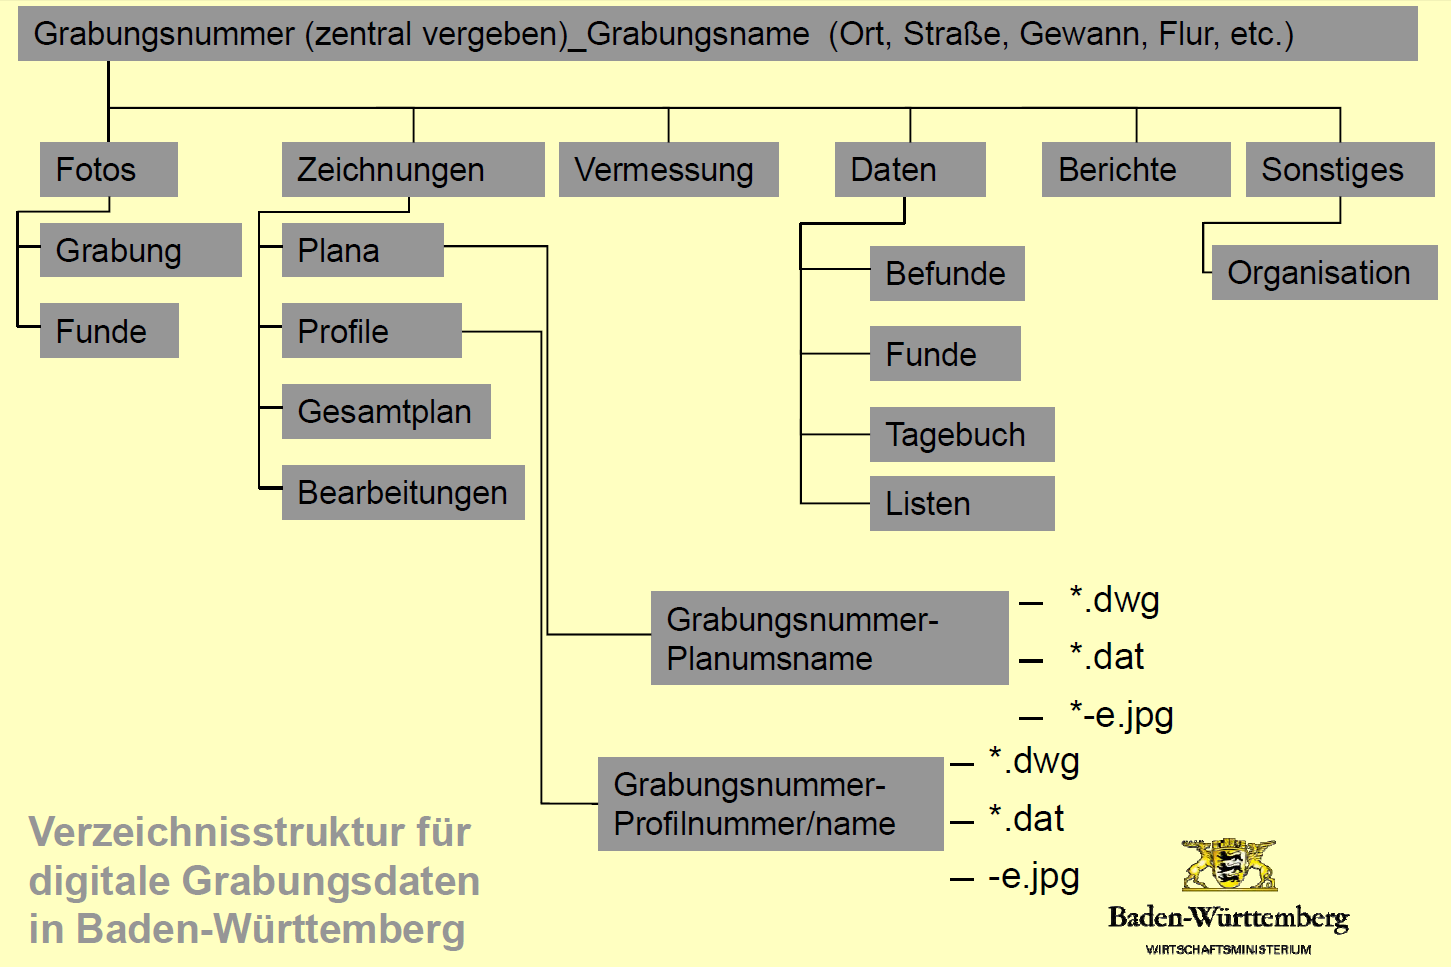
\includegraphics[width=0.9\textwidth]{bilder/OrdnerstrukturBaWue_Bibby}
  \end{center}
  \caption{Datenstruktur Baden-Württemberg}
  \label{OrdnerstrukturBaWue}
\end{figure}

"`\emph{Diese Struktur ist in den oberen Ebenen rigide genug, um für Ordnung und Datendisziplin zu sorgen und gleichzeitig weiter unten flexibel genug, um den unausweichlichen Eigenarten der einzelnen Archäologen Rechnung tragen zu können.}

\emph{Die Grabungs- oder Vorgangsnummer, die zentral vergeben wird, ist wichtig. Sie beschreibt nicht nur die Ausgrabung, sie ist auch die Inventar"=Stammnummer aller Funde, die auf dieser Grabung gefunden werden. Insofern ist sie die Schnittstelle zum zentralen Fundarchiv des Archäologischen Landesmuseums. Die Ausgräber werden aber nicht allein gelassen. Mit der Datenstruktur werden Anleitungen geliefert, die beschreiben, was wohin gehört. Damit wird tatsächlich eine gewisse Einheit im Land erreicht.}"'\footnote{D. Bibby, Digitale Datenstruktur auf Ausgrabungen und Archivierung digitaler Grabungsdaten. Praxis und Praxisversuche aus Baden-Württemberg, ANachr 14 2009, 159-163.}

Auch die nachträgliche Strukturierung von bereits vorhandenen digitalen Dateiablagen ist relativ einfach, da Klartextinhaltsverzeichnisse in der obersten Ebene des Verzeichnisses abgelegt werden können, welche die Eigenheiten der Grabung und die strukturellen Abweichungen beschreiben.

Der Aktenplan des Archäologischen Museums Hamburg wurde für ein analoges Projektarchiv entwickelt, lässt sich jedoch mit wenigen Anpassungen auch gut auf eine digitale Dateiablage anwenden. 

%HAMBURG
\begin{center}
	\begin{longtable}{l l l l}
		\toprule
		\multicolumn{2}{l}{Aktenplan des Archäologischen Museums Hamburg} \\ \midrule \endfirsthead
		\multicolumn{2}{l}{\footnotesize Fortsetzung der vorhergehenden Seite}\\
		\toprule
		\multicolumn{2}{l}{Aktenplan des Archäologischen Museums Hamburg}\\ \midrule \endhead
		\bottomrule \multicolumn{2}{r}{{\footnotesize Fortsetzung auf der nächsten Seite}} \\
		\endfoot
		\bottomrule 
		\endlastfoot
		
		\multicolumn{2}{l}{
\includegraphics[width=0.4cm]{bilder/OrdnerIconZu.png} \hspace*{0.04cm} Datenträger \textit{(nur analog)}}\\
		
		\multicolumn{2}{l}{
\includegraphics[width=0.4cm]{bilder/OrdnerIconAuf.png} \hspace*{0.04cm} Berichte}\\
		& 
\includegraphics[width=0.4cm]{bilder/DateiIcon.png}\hspace*{0.04cm} Grabungsbericht\\
		& 
\includegraphics[width=0.4cm]{bilder/DateiIcon.png} \hspace*{0.04cm} Zwischenberichte\\
		& 
\includegraphics[width=0.4cm]{bilder/DateiIcon.png} \hspace*{0.04cm} Anlagen Zwischenberichte\\
		
		\multicolumn{2}{l}{
\includegraphics[width=0.4cm]{bilder/OrdnerIconAuf.png} \hspace*{0.04cm} Vermessung}\\
	    & 
\includegraphics[width=0.4cm]{bilder/DateiIcon.png} \hspace*{0.04cm} Vermessungspläne\\
		& 
\includegraphics[width=0.4cm]{bilder/DateiIcon.png} \hspace*{0.04cm} Vermessungsunterlagen\\
		& 
\includegraphics[width=0.4cm]{bilder/DateiIcon.png} \hspace*{0.04cm} Vermessungsprotokolle\\
		
		\multicolumn{2}{l}{
\includegraphics[width=0.4cm]{bilder/OrdnerIconAuf.png} \hspace*{0.04cm} Grabungsplänge}\\
	    & 
\includegraphics[width=0.4cm]{bilder/DateiIcon.png} \hspace*{0.04cm} Zeichnungsliste\\
		& 
\includegraphics[width=0.4cm]{bilder/DateiIcon.png} \hspace*{0.04cm} Übersichtpläne\\
		& 
\includegraphics[width=0.4cm]{bilder/DateiIcon.png} \hspace*{0.04cm} Einzelpläne\\
		& 
\includegraphics[width=0.4cm]{bilder/DateiIcon.png} \hspace*{0.04cm} Arbeitspläne\\
		& 
\includegraphics[width=0.4cm]{bilder/DateiIcon.png} \hspace*{0.04cm} Handzeichnungen und Skizzen\\
		
		\multicolumn{2}{l}{
\includegraphics[width=0.4cm]{bilder/OrdnerIconAuf.png} \hspace*{0.04cm} Tagebuch}\\
	    & 
\includegraphics[width=0.4cm]{bilder/DateiIcon.png} \hspace*{0.04cm} Tagebuchausdruck \textit{(oder digitale Datei)}\\
		& 
\includegraphics[width=0.4cm]{bilder/DateiIcon.png} \hspace*{0.04cm} Notizen\\
		
		\multicolumn{2}{l}{
\includegraphics[width=0.4cm]{bilder/OrdnerIconAuf.png} \hspace*{0.04cm} Befunddokumentation}\\
	    & 
\includegraphics[width=0.4cm]{bilder/DateiIcon.png} \hspace*{0.04cm} Befundliste\\
		& 
\includegraphics[width=0.4cm]{bilder/DateiIcon.png} \hspace*{0.04cm} Befundkatalog\\
		& 
\includegraphics[width=0.4cm]{bilder/DateiIcon.png} \hspace*{0.04cm} Notizen\\
		
		\multicolumn{2}{l}{
\includegraphics[width=0.4cm]{bilder/OrdnerIconAuf.png} \hspace*{0.04cm} Funddokumentation}\\
	    & 
\includegraphics[width=0.4cm]{bilder/DateiIcon.png} \hspace*{0.04cm} Fundliste\\
		& 
\includegraphics[width=0.4cm]{bilder/DateiIcon.png} \hspace*{0.04cm} Inventarliste\\
		& 
\includegraphics[width=0.4cm]{bilder/DateiIcon.png} \hspace*{0.04cm} Schriftwechsel\\
		
		\multicolumn{2}{l}{
\includegraphics[width=0.4cm]{bilder/OrdnerIconAuf.png} \hspace*{0.04cm} Probendokumentation}\\
	    & 
\includegraphics[width=0.4cm]{bilder/DateiIcon.png} \hspace*{0.04cm} Probenliste\\
		& 
\includegraphics[width=0.4cm]{bilder/DateiIcon.png} \hspace*{0.04cm} Schriftwechsel\\
		
		\multicolumn{2}{l}{
\includegraphics[width=0.4cm]{bilder/OrdnerIconAuf.png} \hspace*{0.04cm} Fotodokumentation}\\
	    & 
\includegraphics[width=0.4cm]{bilder/DateiIcon.png} \hspace*{0.04cm} Fotoliste\\
		& 
\includegraphics[width=0.4cm]{bilder/DateiIcon.png} \hspace*{0.04cm} Miniaturausdruck \textit{(oder originale Dateien)}\\
		
		\multicolumn{2}{l}{
\includegraphics[width=0.4cm]{bilder/OrdnerIconAuf.png} \hspace*{0.04cm} Dokumente}\\
	    & 
\includegraphics[width=0.4cm]{bilder/DateiIcon.png} \hspace*{0.04cm} Pläne\\
		& 
\includegraphics[width=0.4cm]{bilder/DateiIcon.png} \hspace*{0.04cm} Dokumente und Texte\\
		& 
\includegraphics[width=0.4cm]{bilder/DateiIcon.png} \hspace*{0.04cm} Schriftwechsel\\
		& 
\includegraphics[width=0.4cm]{bilder/DateiIcon.png} \hspace*{0.04cm} Pressespiegel\\
		\bottomrule
	\end{longtable}
\end{center}

Das Bundesdenkmalamt in Österreich hat in seinen Richtlinien eine verpflichtende Ordnerstruktur veröffentlicht, die in einem übergeordneten Ordner mit der Kennung und Benennung der Maßnahme abgelegt wird. Bemerkenswert an dieser Ordnerstruktur ist die sehr flache Hierarchie ohne verschachtelte Ordner, die ein Hinzufügen weiterer benötigter Ordner in der gleichen Ebene zulässt. 

Für die Dateien 01-03 sind in den Richtlinien detaillierte Angaben über den erwarteten Inhalt zu finden. Dies gilt in etwas geringerem Umfang für die übrigen Ordner.  
%ÖSTERREICH
\begin{center}
	\begin{longtable}{l}
		\toprule
		Ordnerstruktur des Bundesdenkmalamtes Österreich \\ \midrule \endfirsthead
		\footnotesize Fortsetzung der vorhergehenden Seite\\
		\toprule
		Ordnerstruktur des Bundesdenkmalamtes Österreich \\ \midrule \endhead
		\bottomrule \multicolumn{1}{r}{{\footnotesize Fortsetzung auf der nächsten Seite}} \\
		\endfoot
		\bottomrule 
		\endlastfoot
		
		
\includegraphics[width=0.4cm]{bilder/DateiIcon.png} \hspace*{0.04cm} 01 Deckblatt\\
		
\includegraphics[width=0.4cm]{bilder/DateiIcon.png} \hspace*{0.04cm} 02 Bericht -- Teil A\\
		
\includegraphics[width=0.4cm]{bilder/DateiIcon.png} \hspace*{0.04cm} 03 Bericht -- Teil B\\
		
\includegraphics[width=0.4cm]{bilder/OrdnerIconZu.png} \hspace*{0.04cm} 04 Technische Daten\\
		
\includegraphics[width=0.4cm]{bilder/OrdnerIconZu.png} \hspace*{0.04cm} 05 SE-Liste \textit{(Liste der Stratigrafischen Einheiten)}\\
		
\includegraphics[width=0.4cm]{bilder/OrdnerIconZu.png} \hspace*{0.04cm} 06 SE-Protokollblätter\\
		\includegraphics[width=0.4cm]{bilder/OrdnerIconZu.png} \hspace*{0.04cm} 07 Objektlisten\\
		\includegraphics[width=0.4cm]{bilder/OrdnerIconZu.png} \hspace*{0.04cm} 08 Objektgruppenlisten \emph{(fakultativ)}\\
		\includegraphics[width=0.4cm]{bilder/OrdnerIconZu.png} \hspace*{0.04cm} 09 Planliste\\
		\includegraphics[width=0.4cm]{bilder/OrdnerIconZu.png} \hspace*{0.04cm} 10 Fundliste\\
		\includegraphics[width=0.4cm]{bilder/OrdnerIconZu.png} \hspace*{0.04cm} 11 Grabungs- bzw. Prospektionsprotokoll\\
		\includegraphics[width=0.4cm]{bilder/OrdnerIconZu.png} \hspace*{0.04cm} 12 Vermessungsunterlagen\\
		\includegraphics[width=0.4cm]{bilder/OrdnerIconZu.png} \hspace*{0.04cm} 13 Originalmessdaten und/oder Metadaten Prospektion\\
		\includegraphics[width=0.4cm]{bilder/OrdnerIconZu.png} \hspace*{0.04cm} 14 Maßnahmenpolygon\\
		\includegraphics[width=0.4cm]{bilder/OrdnerIconZu.png} \hspace*{0.04cm} 15 Technischer Gesamtplan\\
		\includegraphics[width=0.4cm]{bilder/OrdnerIconZu.png} \hspace*{0.04cm} 16 Detailpläne\\
		\includegraphics[width=0.4cm]{bilder/OrdnerIconZu.png} \hspace*{0.04cm} 17 Fotodokumentation\\
		\includegraphics[width=0.4cm]{bilder/OrdnerIconZu.png} \hspace*{0.04cm} 18 Matrix\\
		\includegraphics[width=0.4cm]{bilder/OrdnerIconZu.png} \hspace*{0.04cm} 19 Konservatorische Maßnahmen\\
		\includegraphics[width=0.4cm]{bilder/OrdnerIconZu.png} \hspace*{0.04cm} 20 Sonstige Daten\\
		
		\bottomrule
	\end{longtable}
\end{center}


\hyphenation{
Schnitt-stel-le
}
\label{dateibenennung}
\subsection{Dateibenennung}
Üblicherweise besteht der Dateiname einer Datei aus dem eigentlichen Namen und der durch einen Punkt getrennten Dateinamenserweiterung, die das Format der Datei angibt. Die Erweiterung wird in der Regel von dem Programm, mit dem die Datei gespeichert wurde, automatisch an den Dateinamen gehängt.

Ein Beispiel: \emph{IT-Empfehlungen.pdf} gibt an, dass es sich um eine Datei mit dem Namen \emph{"`IT-Empfehlungen"'} handelt, die in dem PDF-Format vorliegt.

Da die Erweiterung automatisch erzeugt wird, muss die Datei mit einem geeigneten Programm konvertiert werden, wenn man das Dateiformat ändern möchte. In dem Kapitel "`Dateiformate"' ab Seite \pageref{dateiformate} sind ausführliche Informationen darüber zu finden.

Im Folgenden geht es nur noch um den reinen Dateinamen, ohne die Dateinamenserweiterung.

\subparagraph{Erlaubte Zeichen} Moderne Betriebssysteme können mit Sonderzeichen umgehen, zu denen Umlaute und Leerzeichen gehören. Das war aber nicht immer so und kann auch heute noch zu Problemen führen. Webserver lesen zum Beispiel das Leerzeichen als die Zeichenfolge "`$\%20$"' ein und da Umlaute nicht immer gleich kodiert werden, kann auch das zu Schwierigkeiten führen. 

Für die Langzeitarchivierung sollten also nur die alphanumerischen Zeichen des englischen Alphabets, also a-z, A-Z und 0-9 verwendet werden. Zusätzlich kann der Bindestrich ({\bfseries -}) und bei Bedarf auch der Unterstrich ({\bfseries\_}) verwendet werden.

\subparagraph{Zu vermeidende Zeichen} Es gibt eine ganze Reihe von Zeichen, die für besondere Aufgaben von Betriebssystemen verwendet werden. Der Punkt dient zur Trennung des Dateinamens von der Dateinamenserweiterung und der Schrägstrich dient in Windows um Ordnerebenen zu kennzeichnen.

Zu den Zeichen, die absolut nicht verwendet werden dürfen, gehören:
\begin{center}
	\Large \bfseries \textbackslash	 / : * ? "'	< >	|
\end{center}

Die Verwendung von allen weiteren Sonderzeichen ist zwar möglich, kann jedoch zu einem unerwarteten Verhalten des Systems führen. Daher wird von der Verwendung von Leerzeichen und Sonderzeichen, Bindestrich ({\bfseries -}) und Unterstrich ({\bfseries\_}) ausgenommen, abgeraten.

\subparagraph{Groß- und Kleinschreibung} Die Groß- und Kleinschreibung in einem Dateinamen wird von unterschiedlichen Systemen verschieden gedeutet. In Windows beispielsweise kann, wenn es eine Datei mit dem Namen \emph{"`TestDatei"'} schon gibt, keine Datei mit dem Namen \emph{"`testdatei"'} angelegt werden. Andere Systeme könnten dies jedoch erlauben, was aber nicht bedeutet, dass man dies auch tun sollte.

Hat man sich in der Praxis einmal für eine Schreibweise entschieden, muss diese auch konsequent eingehalten werden und insbesondere bei der Arbeit auf verschiedenen Systemen darauf geachtet werden.

\subparagraph{Länge} Der Dateiname sollte so kurz wie möglich und so lang wie nötig sein. Eine aktuelle Obergrenze, die auf manchen Systemen nicht überschritten werden darf, sind 260 Zeichen, wobei dabei der gesamte Dateipfad gezählt wird. Kryptische oder untypische Kürzel sollten vermieden werden, da sie in der Regel in Vergessenheit geraten.

\subsection{Versionskontrolle}\label{versionskontrolle}
Wenn unterschiedliche Personen an einer Datei arbeiten, ist es wichtig, die verschiedenen Änderungen und Entwicklungsstadien zu verfolgen und zu kennzeichnen. Nur so kann vermieden werden, dass an der falschen Dateiversion gearbeitet wird oder diese gar gelöscht wird. Dateiversionen, die nicht mehr benötigt werden, sollten bei Bedarf gelöscht werden.

Es gibt mehrere Strategien, um die Versionskontrolle durchzuführen, die im Folgenden erläutert werden.

\subparagraph{Angabe im Dateinamen} Eine einfache und übersichtliche Methode ist, die Versionsangabe in den Dateinamen zu integrieren. Das kann beispielsweise mit einer Datumsangabe oder Ziffern erfolgen. Durch ein vorangestelltes {\bfseries v} werden die Ziffern als eine Versionsnummer gekennzeichnet, wie zum Beispiel {\bfseries v001}. Führende Nullen stellen sicher, dass die Versionsnummern einheitlich und leichter lesbar sind und richtig sortiert werden.

Eine Kennzeichnung von Versionen durch Worte wie \emph{"`neu"'}, \emph{"`neuer"'} und \emph{"`alt"'} ist unbedingt zu vermeiden. Eine Ausnahme können endgültige Dateiversionen bilden, die der Übersicht halber etwa durch \emph{FINAL} am Ende gekennzeichnet werden können. Es darf aber nur eine Datei mit dieser Kennzeichnung in einem Ordner und einem bestimmten Format vorliegen. Eine endgültige Version, die zum Beispiel sowohl als \emph{docx} als auch als \emph{pdf} vorliegt, ist also erlaubt.

\subparagraph{Angabe in der Datei} Angaben zum Erstellungsdatum und den verschiedenen Versionen und deren Änderungen können im Header der Datei oder in standardisierten Kopfzeilen in der Datei selbst angegeben werden. Bei Textdokumenten bietet sich die Möglichkeit einen Innentitel mit einer Versionshistorie zu verwenden. Ein Beispiel für solch einen Innentitel findet sich am Anfang der PDF-Version dieser Empfehlungen.

\subparagraph{Änderungsprotokoll} Statt einzelne Dateiversionen abzuspeichern, kann auch ein Änderungsprotokoll geführt werden. Dabei werden die einzelnen Änderungen in einer einfachen Textdatei protokolliert, die zusammen mit der eigentlichen Datei abgelegt wird. Im Englischen wird dafür der Begriff \emph{ChangeLog} verwendet.

\subparagraph{Software} Die bisher beschriebenen Methoden sind hauptsächlich manuell anzuwendende Vorgänge. Es gibt jedoch auch Software zur Versionsverwaltung. Deren Einsatz lohnt sich vor allem in großen Projekten, die zentral auf einem Server abgelegt werden. Versionsverwaltungssoftware kann aus den Dateiänderungen automatisch \emph{ChangeLogs} erstellen. Die am weitesten verbreiteten Systeme zur Versionsverwaltung sind \href{http://subversion.apache.org/}{Subversion (SVN)} und \href{https://git-scm.com/}{Git}. Primär wurden sie für die Bedürfnisse von Softwareentwicklern konzipiert, jedoch eignen sie sich auch für allgemeinere Aufgaben. Für die einzelnen Computerarbeitsplätze werden Clients wie \href{https://tortoisesvn.net/}{TortoiseSVN} für SVN oder \href{https://windows.github.com/}{GitHub} für Git benötigt.

Eine einfache Versionsverwaltung für Dateien bieten \href{https://owncloud.org/}{ownCloud}, \href{https://www.dropbox.com/}{Dropbox} und \href{https://drive.google.com/drive/}{Google Drive} wobei die Menge der unterschiedlichen gespeicherten Versionen abhängig von dem persönlichen Speicherplatz ist.

\begin{flushleft}
Git: \urllist{https://git-scm.com/}
Clients für Git: \urllist{https://git-scm.com/downloads/guis}
Subversion (SVN): \urllist{http://subversion.apache.org/}
TortoiseSVN: \urllist{https://tortoisesvn.net/}
ownCloud: \urllist{https://owncloud.org/}
Dropbox: \urllist{https://www.dropbox.com/}
Google Drive: \urllist{https://drive.google.com/drive/}
Vergleich von Versionsverwaltungssystemen auf Wikipedia: \urllist{https://en.wikipedia.org/wiki/Comparison_of_revision_control_software}
\end{flushleft}

\newpage
\section{Dateispeicherung und -sicherung}\label{dateispeicherung}
\abschnittsautor{M. Trognitz, R. Komp, R. Förtsch}
Um Datenverlust vorzubeugen, ist es unerlässlich eine geeignete Sicherungsstrategie zu verwenden. Dabei muss zwischen einer kurzfristigen Speicherung und einer mittelfristigen Sicherung unterschieden werden. Ersteres meint, wie Daten während der Erstellung und Bearbeitung gespeichert werden. Letzteres bezieht sich auf einen längeren Speicherzeitraum, der durchaus auch mehrere Monate betragen kann, stellt also ein klassisches Backup der Daten dar.

Die Sicherungsstrategie legt fest, wie die Datensicherung erfolgen soll und berücksichtigt folgende Fragen:
\begin{itemize}
	\item Wer ist für die Datensicherung verantwortlich?
	\item Wer hat Zugriff auf die gesicherten Daten?
	\item Wann und wie oft soll die Datensicherung durchgeführt werden?
	\item Auf welche Weise soll gesichert werden?
	\item Welche Daten sollen gesichert werden?
	\item Welche Speichermedien sollen verwendet werden?
	\item Wie viele Sicherungskopien sollen angelegt werden?
	\item Wo sollen die Sicherungen aufbewahrt und wie sollen sie geschützt werden?
	\item Wie soll der Transport der Sicherungskopien erfolgen?
	\item Wie lange soll eine Sicherung aufbewahrt werden?
\end{itemize}

Die Sicherungsstrategie kann mit den zu verwendenden Richtlinien zur Dateiablage eng verzahnt sein, um etwa einen nahezu automatisierten Sicherungsvorgang zu ermöglichen.

Die richtige Speicherstrategie beugt zwar möglichen Datenverlusten durch Hardware-, Software- oder menschliche Fehler vor, stellt aber noch \emph{keine} Archivierung der Daten dar. Eine Archivierung ist auf Langfristigkeit ausgelegt und impliziert immer eine bewusste Auswahl und umfassende Dokumentation der Daten, da eine Nachnutzung derselben das Ziel ist. Während der Projektlaufzeit kann bereits ein eigener Archivordner angelegt werden, worin beispielsweise finale Dateien oder unprozessierte Rohdaten abgelegt werden können, um die spätere Auswahl der zu archivierenden Daten vorzubereiten und zu vereinfachen.

Weiterführende Hinweise zur Datensicherung sind auf den Seiten des Bundesamtes für Sicherheit in der Informationstechnik zu finden, die sich sowohl an Einsteiger\footnote{\url{https://www.bsi-fuer-buerger.de/BSIFB/DE/MeinPC/Datensicherung/Sicherungsmethoden/sicherungsmethoden\_node.html}} als auch an Experten\footnote{\url{https://www.bsi.bund.de/DE/Themen/ITGrundschutz/ITGrundschutzKataloge/Inhalt/\_content/baust/b01/b01004.html}} richten. 
\subsection{Kurzfristige Speicherung}
Zur Bearbeitung geöffnete Dateien sollten in kürzeren Abständen gespeichert werden, um einem Verlust von stundenlanger Arbeit infolge etwa eines Stromausfalls vorzubeugen. Von diesen Arbeitsversionen sollten regelmäßig, beispielsweise nach jedem Arbeitstag, Kopien auf externen Speichermedien angefertigt werden, welche in die mittelfristige Sicherung übergehen.

Vorgaben zur Form der Dateiablage, der Dateibenennung und Versionierung müssen schon beim Anlegen der Dateien beachtet werden, um einen reibungslosen Ablauf der darauf abgestimmten Datensicherungsstrategie zu gewährleisten. Hinweise dazu sind im Abschnitt Dateiverwaltung ab Seite \pageref{dateiverwaltung} zu finden.

\subsection{Mittelfristige Sicherung}
Digitale Daten sind nur dann über einen längeren Zeitraum sicher, wenn sie mehr als einmal gespeichert werden. Es müssen also mindestens zwei Sicherungskopien auf physisch getrennten Speichermedien vorliegen, um etwa bei einem Hardwaredefekt auf eine alternative Sicherungskopie zugreifen zu können.

Die Sicherung von Daten auf unterschiedlichen Arbeitsgeräten wird erleichtert, wenn diese zunächst auf einem Datenträger gesammelt werden und dieser dann gesichert wird.

\subparagraph{Speichermedium} Welches Speichermedium gewählt wird, hängt vor allem von der Speichergröße der zu sichernden Dateien und der vorhandenen Infrastruktur ab. So eignen sich eine CD oder eine DVD nur für Daten bis maximal 900 MB bzw. 17 GB Speichervolumen. Für größere Datenmengen werden entsprechend größere Datenträger benötigt. 

Steht ein lokaler oder institutioneller Server zur Verfügung, sollte dieser zur Datensicherung verwendet werden, da diese üblicherweise gewartet werden und meist selbst in eigene Sicherungsstrategien eingebunden sind. In Umgebungen mit Zugriff auf das Internet, kann eine Sicherung auch auf einen entfernten Server, beispielsweise in einem Rechenzentrum, erfolgen. In allen anderen Fällen können externe Festplatten verwendet werden. Von externen kommerziellen Diensten, wie beispielsweise Dropbox, ist für eine mittelfristige Sicherung abzuraten, weil es sich oft um ausländische Anbieter handelt, die nicht dem deutschen Recht unterliegen und den Nutzer im Unklaren darüber lassen, wie mit den Daten umgegangen wird.

Da die Speichermedien eine begrenzte Lebenszeit von etwa zehn Jahren haben, sollten die Sicherungen von Zeit zu Zeit auf neue Speichermedien migriert werden. Außerdem sollten sie zwischenzeitlich an verschiedenen Orten, mindestens in verschiedenen Räumen, gelagert werden, um etwa im Brandfall den Schaden zu begrenzen. Auch der Transport von Original- und Sicherungsdatenbeständen sollte getrennt durch unterschiedliche Personen erfolgen, um zu vermeiden, dass etwa durch Diebstahl alle Sicherungskopien auf einmal abhanden kommen. 

Für das Kopieren der Daten auf ein Speichermedium gibt es verschiedene Methoden, wie die im Folgenden beschriebene Volldatensicherung, inkrementelle und differentielle Datensicherung.

\subparagraph{Volldatensicherung} Bei der Volldatensicherung werden die zu sichernden Dateien komplett und eins zu eins auf ein Speichermedium kopiert. Wird zum ersten Mal eine Sicherungskopie angelegt, so muss dies als Volldatensicherung geschehen. Dabei ist zu beachten, dass der Kopiervorgang viel Zeit in Anspruch nehmen kann, wobei dies auch über Nacht geschehen kann. Vor der Ausführung der Volldatensicherung muss geprüft werden, dass auf dem Speichermedium ausreichend freier Speicherplatz vorhanden ist. 

Die Volldatensicherung ist die einzige Methode, die manuell, ohne weitere Hilfsprogramme, durchgeführt werden kann. Wird eine Volldatensicherung angelegt, sollten, beispielsweise in einer Textdatei, Informationen gespeichert werden, die Auskunft über den Zeitpunkt der Sicherung, den Ansprechpartner und den Umfang der Daten geben.

Liegt eine erste Volldatensicherung vor, können neue oder geänderte Daten mittels inkrementeller oder differentieller Datensicherung gesichert werden, was die Möglichkeit bietet, verschiedene Versionen der Daten zu sichern. Für beide Methoden werden jedoch eigene Programme benötigt.

\subparagraph{Inkrementelle Sicherung} Die inkrementelle Sicherung speichert nur jene Daten, die sich im Vergleich zu der vorliegenden Volldatensicherung oder vergangenen inkrementellen Sicherungsvorgängen geändert haben. Dies spart Zeit und Speicherplatz, erfordert jedoch im Fall einer Wiederherstellung der Daten, dass zunächst die Volldatensicherung übertragen wird und anschließend alle erfolgten inkrementellen Sicherungen nacheinander eingespielt werden.

\subparagraph{Differentielle Sicherung} Bei der differentiellen Sicherung werden immer jene Daten gespeichert, die sich im Verlgeich zu der vorliegenden letzten Volldatensicherung geändert haben. Im Unterschied zu der inkrementellen Sicherung entfällt also der Vergleich mit Daten aus zwischenliegenden Sicherungsvorgängen seit Erstellung der Volldatensicherung. Diese Methode erfordert zwar etwas mehr Zeit und Speicherplatz als die inkrementelle Sicherung, erleichtert aber die Wiederherstellung der Daten, da nur die Volldatensicherung und die letzte differentielle Sicherung auf das System übertragen werden muss. Die vorherigen differentiellen Sicherungen werden nicht benötigt.

\subparagraph{Automatisierung} Die Datensicherung kann mit Hilfe von Programmen oder Skripten automatisiert erfolgen. Wichtig ist dabei zu kontrollieren, dass die Datensicherung auch tätsächlich in der gewünschten Form ausgeführt wird. Geeignete Programme gibt es viele, wie beispielsweise \href{http://bacula.org/}{Bacula}, \href{http://www.dirsyncpro.org/}{DirSync Pro}, \href{http://www.traybackup.de}{TrayBackup}, \href{http://personal-backup.rathlev-home.de}{PersonalBackup} oder \href{http://rsync.samba.org/}{rsync}. Eine ausführliche Liste ist außerdem auf der englischen Wikipedia unter \href{http://en.wikipedia.org/wiki/List\_of\_backup\_software}{List of backup software} zu finden. Oft können die Programme auch zur Wiederherstellung von gesicherten Daten verwendet werden.

\begin{flushleft}
	DirSync Pro: \urllist{http://www.dirsyncpro.org/}
	TrayBackup: \urllist{http://www.traybackup.de}
	PersonalBackup: \urllist{http://personal-backup.rathlev-home.de}
	rsync: \urllist{http://rsync.samba.org/}
	Liste von Backup-Programmen auf Wikipedia: \urllist{http://en.wikipedia.org/wiki/List_of_backup_software} 
\end{flushleft}

\subparagraph{Sicherungszeitpunkt} Der Zeitpunkt der Sicherung spielt eine nicht zu unterschätzende Rolle. Beispielsweise kann eine Sicherung von Datenbanken im laufenden Betrieb zu Inkonsistenzen führen, weshalb in solchen Fällen ein Administrator diese Aufgabe übernehmen sollte.

Regelmäßige Sicherungsvorgänge, die zu bestimmten Zeitpunkten täglich, wöchentlich oder monatlich automatisiert gestartet und durchlaufen werden, gewährleisten, dass eine Sicherung auch tatsächlich erfolgt, zumal sie nicht vom individuellen Verhalten eines Nutzers abhängen.

Für Daten, die verschiedene Arbeitsschritte durchlaufen und dadurch große Änderungen erfahren, können die verschiedenen Zustände als Sicherungspunkte gespeichert werden. Beispielsweise können zunächst unbearbeitete digitale Bilder gespeichert werden, sowie ein daraus erzeugtes photogrammetrisches Modell oder andere nicht oder nur schwer reproduzierbare signifikante Verarbeitungsschritte. Solche Sicherungspunkte müssen allerdings manuell gemacht werden, indem beispielsweise ein Ordner mit den Rohdaten angelegt wird. Hinweise für solche Sicherungspunkte werden für bestimmte angewendete Methoden in dem Kapitel Forschungsmethoden ab Seite \pageref{methoden} gegeben.

\subparagraph{Sicherungsversionen} Es empfiehlt sich, eine vorhandene Volldatensicherung nicht direkt mit einer neuen Volldatensicherung zu überschreiben. Tritt nämlich während des Sicherungsvorganges ein Fehler auf, könnte auch die bereits vorhandene Sicherungsversion beschädigt werden.

Bei der Anwendung von inkrementellen oder differentiellen Sicherungsmethoden sollte trotzdem in geregelten Zeitabständen eine neue Volldatensicherung angelegt werden, welche mindestens bis zur nächsten Volldatensicherung aufgehoben wird. Dies ist im Sinne des Generationenprinzips oder Großvater-Vater-Sohn-Prinzips, einer Strategie zur Datensicherung, bei der mehrere Sicherungen für verschiedenen Zeitpunkte und Zwecke angelegt werden. Hierfür können beispielsweise wöchentlich und monatlich Volldatensicherungen angelegt werden (Vater und Großvater), die primär den Datenverlust durch Hardware- oder Software-Fehler reduzieren sollen. Tägliche inkrementelle oder differentielle Sicherungen (Sohn) erlauben es beispielsweise auf Arbeitsversionen des Vortages zuzugreifen und können mit dem Beginn einer neuen Woche nach und nach überschrieben werden. 

\subparagraph{Disaster Recovery} Eine gute Sicherungsstrategie umfasst zusätzlich die Erprobung der Wiederherstellung der Daten, um im Ernstfall sicher zu sein, dass die verwendete Strategie auch wirklich funktioniert und die Daten schnell wieder einsatzfähig sind. Somit können vorhandene Sicherungsversionen ebenfalls auf ihre Funktionsfähigkeit überprüft werden.